% Options for packages loaded elsewhere
% Options for packages loaded elsewhere
\PassOptionsToPackage{unicode}{hyperref}
\PassOptionsToPackage{hyphens}{url}
\PassOptionsToPackage{dvipsnames,svgnames,x11names}{xcolor}
%
\documentclass[
  british,
  a4paper,
  DIV=11,
  numbers=noendperiod]{scrreprt}
\usepackage{xcolor}
\usepackage[margin=1in]{geometry}
\usepackage{amsmath,amssymb}
\setcounter{secnumdepth}{5}
\usepackage{iftex}
\ifPDFTeX
  \usepackage[T1]{fontenc}
  \usepackage[utf8]{inputenc}
  \usepackage{textcomp} % provide euro and other symbols
\else % if luatex or xetex
  \usepackage{unicode-math} % this also loads fontspec
  \defaultfontfeatures{Scale=MatchLowercase}
  \defaultfontfeatures[\rmfamily]{Ligatures=TeX,Scale=1}
\fi
\usepackage{lmodern}
\ifPDFTeX\else
  % xetex/luatex font selection
\fi
% Use upquote if available, for straight quotes in verbatim environments
\IfFileExists{upquote.sty}{\usepackage{upquote}}{}
\IfFileExists{microtype.sty}{% use microtype if available
  \usepackage[]{microtype}
  \UseMicrotypeSet[protrusion]{basicmath} % disable protrusion for tt fonts
}{}
\makeatletter
\@ifundefined{KOMAClassName}{% if non-KOMA class
  \IfFileExists{parskip.sty}{%
    \usepackage{parskip}
  }{% else
    \setlength{\parindent}{0pt}
    \setlength{\parskip}{6pt plus 2pt minus 1pt}}
}{% if KOMA class
  \KOMAoptions{parskip=half}}
\makeatother
% Make \paragraph and \subparagraph free-standing
\makeatletter
\ifx\paragraph\undefined\else
  \let\oldparagraph\paragraph
  \renewcommand{\paragraph}{
    \@ifstar
      \xxxParagraphStar
      \xxxParagraphNoStar
  }
  \newcommand{\xxxParagraphStar}[1]{\oldparagraph*{#1}\mbox{}}
  \newcommand{\xxxParagraphNoStar}[1]{\oldparagraph{#1}\mbox{}}
\fi
\ifx\subparagraph\undefined\else
  \let\oldsubparagraph\subparagraph
  \renewcommand{\subparagraph}{
    \@ifstar
      \xxxSubParagraphStar
      \xxxSubParagraphNoStar
  }
  \newcommand{\xxxSubParagraphStar}[1]{\oldsubparagraph*{#1}\mbox{}}
  \newcommand{\xxxSubParagraphNoStar}[1]{\oldsubparagraph{#1}\mbox{}}
\fi
\makeatother


\usepackage{longtable,booktabs,array}
\usepackage{calc} % for calculating minipage widths
% Correct order of tables after \paragraph or \subparagraph
\usepackage{etoolbox}
\makeatletter
\patchcmd\longtable{\par}{\if@noskipsec\mbox{}\fi\par}{}{}
\makeatother
% Allow footnotes in longtable head/foot
\IfFileExists{footnotehyper.sty}{\usepackage{footnotehyper}}{\usepackage{footnote}}
\makesavenoteenv{longtable}
\usepackage{graphicx}
\makeatletter
\newsavebox\pandoc@box
\newcommand*\pandocbounded[1]{% scales image to fit in text height/width
  \sbox\pandoc@box{#1}%
  \Gscale@div\@tempa{\textheight}{\dimexpr\ht\pandoc@box+\dp\pandoc@box\relax}%
  \Gscale@div\@tempb{\linewidth}{\wd\pandoc@box}%
  \ifdim\@tempb\p@<\@tempa\p@\let\@tempa\@tempb\fi% select the smaller of both
  \ifdim\@tempa\p@<\p@\scalebox{\@tempa}{\usebox\pandoc@box}%
  \else\usebox{\pandoc@box}%
  \fi%
}
% Set default figure placement to htbp
\def\fps@figure{htbp}
\makeatother


% definitions for citeproc citations
\NewDocumentCommand\citeproctext{}{}
\NewDocumentCommand\citeproc{mm}{%
  \begingroup\def\citeproctext{#2}\cite{#1}\endgroup}
\makeatletter
 % allow citations to break across lines
 \let\@cite@ofmt\@firstofone
 % avoid brackets around text for \cite:
 \def\@biblabel#1{}
 \def\@cite#1#2{{#1\if@tempswa , #2\fi}}
\makeatother
\newlength{\cslhangindent}
\setlength{\cslhangindent}{1.5em}
\newlength{\csllabelwidth}
\setlength{\csllabelwidth}{3em}
\newenvironment{CSLReferences}[2] % #1 hanging-indent, #2 entry-spacing
 {\begin{list}{}{%
  \setlength{\itemindent}{0pt}
  \setlength{\leftmargin}{0pt}
  \setlength{\parsep}{0pt}
  % turn on hanging indent if param 1 is 1
  \ifodd #1
   \setlength{\leftmargin}{\cslhangindent}
   \setlength{\itemindent}{-1\cslhangindent}
  \fi
  % set entry spacing
  \setlength{\itemsep}{#2\baselineskip}}}
 {\end{list}}
\usepackage{calc}
\newcommand{\CSLBlock}[1]{\hfill\break\parbox[t]{\linewidth}{\strut\ignorespaces#1\strut}}
\newcommand{\CSLLeftMargin}[1]{\parbox[t]{\csllabelwidth}{\strut#1\strut}}
\newcommand{\CSLRightInline}[1]{\parbox[t]{\linewidth - \csllabelwidth}{\strut#1\strut}}
\newcommand{\CSLIndent}[1]{\hspace{\cslhangindent}#1}

\ifLuaTeX
\usepackage[bidi=basic]{babel}
\else
\usepackage[bidi=default]{babel}
\fi
% get rid of language-specific shorthands (see #6817):
\let\LanguageShortHands\languageshorthands
\def\languageshorthands#1{}
\ifLuaTeX
  \usepackage[english]{selnolig} % disable illegal ligatures
\fi


\setlength{\emergencystretch}{3em} % prevent overfull lines

\providecommand{\tightlist}{%
  \setlength{\itemsep}{0pt}\setlength{\parskip}{0pt}}



 


\KOMAoption{captions}{tableheading}
\makeatletter
\@ifpackageloaded{caption}{}{\usepackage{caption}}
\AtBeginDocument{%
\ifdefined\contentsname
  \renewcommand*\contentsname{Table of contents}
\else
  \newcommand\contentsname{Table of contents}
\fi
\ifdefined\listfigurename
  \renewcommand*\listfigurename{List of Figures}
\else
  \newcommand\listfigurename{List of Figures}
\fi
\ifdefined\listtablename
  \renewcommand*\listtablename{List of Tables}
\else
  \newcommand\listtablename{List of Tables}
\fi
\ifdefined\figurename
  \renewcommand*\figurename{Figure}
\else
  \newcommand\figurename{Figure}
\fi
\ifdefined\tablename
  \renewcommand*\tablename{Table}
\else
  \newcommand\tablename{Table}
\fi
}
\@ifpackageloaded{float}{}{\usepackage{float}}
\floatstyle{ruled}
\@ifundefined{c@chapter}{\newfloat{codelisting}{h}{lop}}{\newfloat{codelisting}{h}{lop}[chapter]}
\floatname{codelisting}{Listing}
\newcommand*\listoflistings{\listof{codelisting}{List of Listings}}
\makeatother
\makeatletter
\makeatother
\makeatletter
\@ifpackageloaded{caption}{}{\usepackage{caption}}
\@ifpackageloaded{subcaption}{}{\usepackage{subcaption}}
\makeatother
\usepackage{bookmark}
\IfFileExists{xurl.sty}{\usepackage{xurl}}{} % add URL line breaks if available
\urlstyle{same}
\hypersetup{
  pdftitle={Mixed cropping of narrow‑leaved lupin with oat enhances grain‑yield stability across five European locations},
  pdflang={en-GB},
  colorlinks=true,
  linkcolor={blue},
  filecolor={Maroon},
  citecolor={Blue},
  urlcolor={Blue},
  pdfcreator={LaTeX via pandoc}}


\title{Mixed cropping of narrow‑leaved lupin with oat enhances
grain‑yield stability across five European locations}
\author{}
\date{2026-03-20, 18:18}
\begin{document}
\maketitle

\renewcommand*\contentsname{Table of contents}
{
\hypersetup{linkcolor=}
\setcounter{tocdepth}{2}
\tableofcontents
}

\textbf{Yannik Schlup¹ ³}✉, \textbf{Vesna Župunski²}, \textbf{Radivoje
Jevtić²}, \textbf{Selma Schurack⁴},\\
\textbf{Matthias Heinrich Herrmann⁴},\\
\textbf{Andrea Gallehr⁵},\\
\textbf{Kathrin Neubeck⁵}, \textbf{Annette Haak⁵},\\
\textbf{Lukas Graz⁶},\\
\textbf{Johan Six³},\\
\textbf{Susanne Vogelgsang¹}✉

¹ Research group Extension Arable Crops, Competence Division Plant and
Plant Products, Agroscope, Zurich, Switzerland\\
² Institute of Field and Vegetable Crops, Novi Sad, Serbia ³ Sustainable
Agroecosystems, Department of Environmental Systems Science, ETH Zurich,
Zurich, Switzerland ⁴ Institute for Breeding Research on Agricultural
Crops, Julius Kühn Institute (JKI), Federal Research Centre for
Cultivated Plants, Sanitz, Germany ⁵ Research \& Breeding department
(FZD) at Landbauschule Dottenfelderhof, Bad Vilbel, Germany ⁶ Seminar
for Statistics, Department of Mathematics, ETH Zurich, Zurich,
Switzerland

✉ Corresponding authors: schlupy@ethz.ch,
susanne.vogelgsang@agroscope.admin.ch

\chapter{Abstract}\label{abstract}

\textbf{Background \& aims:} Pulse x cereal mixtures are promoted to
stabilise yield and reduce fertiliser dependence, yet robust
multi‑environment evidence for narrow‑leaved lupin (NLL, \emph{Lupinus
angustifolius}) × oat (\emph{Avena sativa}) mixed cropping remains
scarce. We tested whether NLL × oat mixtures maintain productivity while
enhancing grain yield stability.

\textbf{Methods:} A randomised complete block design (four blocks)
evaluated three NLL and three oat varieties grown as pure stands and as
all nine pairwise mixtures in a replacement design (NLL 90\%, oat 10\%
of pure‑stand density). The experiments ran for 13 environment‑years
across five European locations. Productivity was summarised with land
equivalent ratio (LER) and crop performance ratio (CPR). Yield stability
was assessed using (i) the coefficient of variation (CV), (ii)
Finlay-Wilkinson regression slope (\(b_{1}\)) and Eberhart--Russell
deviation variance (\(S^2_{di}\)), and (iii) additive main effects and
multiplicative interaction‑derived weighted average of absolute scores
(AMMI-WAAS). Mixed‑effects models were used to assess mixed cropping
effects.

\textbf{Results:} Across environments, LER did not differ from unity
(LER = 1) whether fertilised or unfertilised oat monocultures were the
reference. By contrast, total CPR and oat specific CPR consistently
exceeded 1 (mean CPR = 5.3; CPR\_N = 4.6), indicating system level gains
driven by the oat component without penalising NLL. While CVs did not
separate treatments, many mixtures and pure stands were environmentally
responsive, but the most stable mixtures combined near average
responsiveness with very low variation and sensitivity to the
environmental conditions (Bison × Probor and Troll × Jowisz). Lastly,
fertilised oat monocultures were more stable than unfertilised
counterparts.

\textbf{Conclusions:} Stability gains arose from reduced environmental
sensitivity of the mixture rather than the individual variety,
underscoring the need to evaluate mixtures directly rather than
inferring stability from monocultures. These results support deploying
pulse‑centric cereal × legume mixtures as a pragmatic option to buffer
climate variability while sustaining protein‑rich production.

\textbf{Keywords}: mixed cropping, \emph{Lupinus angustifolius},
\emph{Avena sativa}, LER, CPR, Finlay--Wilkinson, AMMI, WAAS, yield
stability, genotype × environment.

\chapter{Introduction}\label{introduction}

Global demand for protein‐rich plants is growing while climate
volatility continues to undermine the year‑to‑year reliability of
monocultures (Ismail et al., 2020; Raseduzzaman and Jensen, 2017). Mixed
cropping of cereals with grain legumes (pulses) has re‑emerged as a
promising strategy to improve yield stability, decrease fertiliser
dependence and improve resource‑use efficiency (Kumawat et al., 2022;
Raseduzzaman and Jensen, 2017; Rodriguez et al., 2020; Tang et al.,
2021). Narrow‑leaved lupin\,(NLL, \emph{Lupinus angustifolius} L.) is
among the few pulses that combine high seed protein with the ability to
thrive on nutrient poor soils (Lopez-Bellido and Fuente, 1986); however,
its sole‑crop yield is notoriously unstable (Reckling et al., 2018).
Oat\,(\emph{Avena sativa} L.) offers complementary morphology, rapid
early growth and serves as a cereal break crop (e.g. Danso et al., 1993;
Pálmason et al., 1992). Integrating the two species in mixed cropping
can therefore address both agronomic resilience and nutritional targets
at farm and food‑system level, respectively.

Numerous studies on genotype × cropping‑system interactions have
demonstrated that performance gains from cereal × pulse mixtures depend
on both the mixed varieties and the environment in which they were
evaluated (e.g. (Demie et al., 2022)). Meta‑analyses consistently report
average land‑equivalent ratios (LER) between 1.2 and 1.3 for
cereal-pulse mixtures, indicating a median 24\% land‑use advantage over
pure stands (Demie et al., 2022). Grain-yield stability has been
assessed with both static and dynamic metrics; in many cases, mixtures
outperformed monocultures, yet the magnitude and drivers of this
stability remain unclear (Raseduzzaman and Jensen, 2017; Weih et al.,
2021).

Fertiliser regimes of cereals in pure stands are pivotal for
interpreting mixed‑cropping metrics because both LER and crop
performance ratio (CPR) are normalised by monoculture benchmarks
(Hauggaard-Nielsen and Jensen, 2001; Liu et al., 2023). In formal terms,
the CPR compares observed mixed cropping output to the output expected
from monoculture yields at the same sowing proportions (Zustovi et al.,
2024). As a consequence of fertilising cereals in pure stands and the
resulting increase in yield, the denominator of the cereal LER and CPR
raises, which results in lower LER and CPR-metrics for the same mixed
crop. Though rarely investigated, reference treatment fertilisation
exhibits significant effects on the mixed cropping performance metrics
(Baxevanos et al., 2020). Additionally, medium to high fertiliser levels
were shown to stabilise cereal yield (Silva et al., 2016). Thus, the
choice of baseline (fertilised vs.~unfertilised) pure cereal stands
directly affects mixed‑cropping advantages in terms of productivity and
stability metrics (Li et al., 2020; Mead and Willey, 1980).

Despite this theory, robust multi‑environment evidence for NLL × oat
mixtures is scarce. Previous experiments have often been confined to
single locations, or ad‑hoc varietal choices, leaving unresolved (i)
whether crop‑level indices such as the CPR validate classical LER
assessments, (ii) how canopy height difference between the varieties
influence the agronomic performance, (iii) whether the expected
grain-yield stability gains of mixed cropping materialise across
contrasting European agroclimates and (iv) how fertilisation of the pure
reference cereal crop affects yield indices and stability metrics in
mixed stands. Addressing these gaps is critical, since pulses are
pivotal to climate‑change mitigation strategies and nitrogen‑fertiliser
reduction programmes (Rahman et al., 2022).

Accordingly, we expect

- Mixed stands to achieve LER values above\,1, indicating superior land
use compared with pure stands

- Total CPR and the oat CPR to exceed unity (CPR above 1), reflecting an
overall mixed cropping advantage

\begin{itemize}
\tightlist
\item
  The CPR and LER to be relatively smaller if those metrics are compared
  with fertilised rather than unfertilised pure stands of oats
\end{itemize}

- NLL × oat mixed cropping to increase both static and dynamic
grain-yield stability across the five European locations relative to
their corresponding pure stands and

\begin{itemize}
\tightlist
\item
  The gain in grain-yield stability of mixed stands to be relatively
  smaller if that gain is compared with fertilised rather than
  unfertilised pure stands of oats.
\end{itemize}

\chapter{Methods}\label{methods}

\section{Varieties}\label{varieties}

Three branching spring NLL and three spring oat varieties were chosen
based on the breeders' fact sheets and the variety list of the German
variety institute (Bundessortenamt, 2021). Branching, spring-NLLs and
early maturing spring oat varieties were selected to increase the
chances of coincidental ripening. The selected, NLL varieties were

\begin{itemize}
\tightlist
\item
  Lunabor, bred by Saatzucht Steinach in Germany
\item
  Probor, bred by Saatzucht Steinach in Germany
\item
  Jowisz (synonym: Jupiter), bred by HR Smolic in Poland
\end{itemize}

The selected early maturing spring oat varieties were:

\begin{itemize}
\tightlist
\item
  Bison, Hauptsaaten für die Rheinprovinz GmbH, Germany, medium tall
\item
  Lion, Nordsaat Saatzucht GmbH, Germany, medium tall
\item
  Troll, Saatzucht Bauer GmbH \& Co.~KG, Germany, short.
\end{itemize}

\section{Treatments and experimental
design}\label{treatments-and-experimental-design}

The NLL and oat varieties were cultivated as spring crops in pure and
mixed stands. The pure oat stands were fertilised according to the local
guidelines (Supplemental materials - Table S1). In the mixed stands,
each NLL variety was co-cultivated with each oat variety in a
replacement design: the NLLs were sown at 90\% of their pure stand's
density, whereas the oats, due to their high competitiveness and the
focus on the NLL crop, were sown at 10\% of their pure stand's density
(Böhm et al., 2008; Kato-Noguchi et al., 1994) (\hyperref[tbl_trt]{Table
1}). The sowing amounts were adapted to the germination rate.

\begin{table}

\caption{\label{tbl-trt}}

\centering{

Treatments of the study: narrow-leaved lupin and oat varieties, the
stand (pure versus mixed), fertilisation, sowing ratios, respective
sowing densities and corresponding amount of seeds per hectare. For the
two numbers presented in the mixed treatments, the first one refers to
the narrow-leaved lupins, the second one to the oats. The sowing density
and fertilisation of the oat crop varied depending on the local
recommendations.

}

\end{table}%

\begin{longtable}[]{@{}
  >{\raggedright\arraybackslash}p{(\linewidth - 8\tabcolsep) * \real{0.2093}}
  >{\raggedright\arraybackslash}p{(\linewidth - 8\tabcolsep) * \real{0.1047}}
  >{\raggedright\arraybackslash}p{(\linewidth - 8\tabcolsep) * \real{0.1744}}
  >{\raggedright\arraybackslash}p{(\linewidth - 8\tabcolsep) * \real{0.3256}}
  >{\raggedright\arraybackslash}p{(\linewidth - 8\tabcolsep) * \real{0.1860}}@{}}
\toprule\noalign{}
\begin{minipage}[b]{\linewidth}\raggedright
Treatment
\end{minipage} & \begin{minipage}[b]{\linewidth}\raggedright
Stand
\end{minipage} & \begin{minipage}[b]{\linewidth}\raggedright
Fertilisation*
\end{minipage} & \begin{minipage}[b]{\linewidth}\raggedright
Sowing density** (plantsm\textsuperscript{-2})
\end{minipage} & \begin{minipage}[b]{\linewidth}\raggedright
Amount (kgha\textsuperscript{-1})
\end{minipage} \\
\midrule\noalign{}
\endhead
\bottomrule\noalign{}
\endlastfoot
Bison & pure & no & 300 - 400 & 168 - 224 \\
Lion & pure & no & 300 - 400 & 121 - 161 \\
Troll & pure & no & 300 - 400 & 110 - 147 \\
Bison & pure & yes & 300 - 400 & 168 - 224 \\
Lion & pure & yes & 300 - 400 & 121 - 161 \\
Troll & pure & yes & 300 - 400 & 110 - 147 \\
Lunabor & pure & no & 120 & 220 \\
Probor & pure & no & 120 & 170 \\
Jowisz & pure & no & 120 & 214 \\
Lunabor × Bison & mixed & no & 108 / 30 - 40 & 198 / 17 - 22 \\
Lunabor × Lion & mixed & no & 108 / 30 - 40 & 198 / 12 - 16 \\
Lunabor × Troll & mixed & no & 108 / 30 - 40 & 198 / 11 - 15 \\
Probor × Bison & mixed & no & 108 / 30 - 40 & 153 / 17 - 22 \\
Probor × Lion & mixed & no & 108 / 30 - 40 & 153 / 12 - 16 \\
Probor × Troll & mixed & no & 108 / 30 - 40 & 153 / 11 - 15 \\
Jowisz × Bison & mixed & no & 108 / 30 - 40 & 193 / 17 - 22 \\
Jowisz × Lion & mixed & no & 108 / 30 - 40 & 193 / 12 - 16 \\
Jowisz × Troll & mixed & no & 108 / 30 - 40 & 193 / 11 - 15 \\
\end{longtable}

*Fertilisation was performed according to local guidelines (Supplemental
materials - Table S1). **Novi Sad: 400 plants·m\textsuperscript{-2}, Bad
Vilbel and Gross Lüewitz: 350 plants·m\textsuperscript{-2}, Reckenholz
and Seegräben: 300 plants·m\textsuperscript{-2}

The fields of this two-year study were arranged as a randomised complete
block design (RCBD), consisting of four blocks. To lower the border
effect to a minimum, each treatment was sown in three adjacent plots and
only the middle plot was scored and harvested. The size of each
harvested plot was 9m\textsuperscript{2}.

\section{Locations, husbandry and weather
data}\label{locations-husbandry-and-weather-data}

The experiments were conducted in Germany (Bad Vilbel and Gross
Lüsewitz), Serbia (Novi Sad) and in Switzerland (Seegräben and
Reckenholz) and were chosen based on their differing latitude,
longitude, soil type (Supplemental materials - Table S1) and weather
conditions (Table 2). In Switzerland, the experiments were performed in
2022 and 2023, while in Serbia and Germany, they were conducted in 2022,
2023 and 2024. All fields were ploughed and harrowed before sowing. The
NLL seeds were inoculated with peat inoculum containing the rhizobium
bacterium \emph{Bradyrhizobium lupinus}. The inoculum was produced by
Legume Technology Ltd, Nottinghamshire, UK. The same batch of inoculum
was used in all years and stored dry and under exclusion of humidity at
10°C. After the inoculation, every 9m\textsuperscript{2} plot was sown
individually in rows with 18 cm spacing. The plots were sown with a plot
sowing tractor and RTK-GPS-orientation. Spring-tine and shallow
inter-row cultivation was performed for the mechanical weeding. Chemical
weed control was applied only at Gross Lüsewitz in 2022 and 2024 using
the pre-emergence herbicide Stomp Aqua; at all other sites, weeds were
controlled mechanically or manually, or no weeding was required
(Supplementary Materials - Table S1). The fertilised pure oats were
fertilised during late tillering, before the elongation stage, according
to local guidelines (Supplemental materials - Table S1). At Bad Vilbel,
following organic production principles, horn grit was used as
fertiliser.

\begin{table}

\caption{\label{tbl-weather}}

\centering{

Weather data of the location and year in the cultivation seasons 2022,
2023 and 2024 (13 environment-years), retrieved from the closest
official weather stations (the distance of the weather station to the
location was between 0.25 and 5 km). Data were retrieved daily and the
average temperature as well as the sum of precipitation across the
location- and year-specific cultivation period were calculated.

}

\end{table}%

\begin{longtable}[]{@{}lll@{}}
\toprule\noalign{}
Location and year & Mean temperature (°C) & Precipitation sum (mm) \\
\midrule\noalign{}
\endhead
\bottomrule\noalign{}
\endlastfoot
Bad Vilbel 2022 & 13.4 & 174 \\
Bad Vilbel 2023 & 13.1 & 293 \\
Bad Vilbel 2024 & 13.8 & 402 \\
Gross Lüsewitz 2022 & 11.8 & 234 \\
Gross Lüsewitz 2023 & 11.8 & 258 \\
Gross Lüsewitz 2024 & 13 & 367 \\
Novi Sad 2022 & 22.7 & 75 \\
Novi Sad 2023 & 17.8 & 234 \\
Novi Sad 2024 & 17.4 & 175 \\
Seegräben 2022 & 14.1 & 504 \\
Seegräben 2023 & 13.8 & 500 \\
Reckenholz 2022 & 17.7 & 244 \\
Reckenholz 2023 & 17.4 & 362 \\
\end{longtable}

\section{Harvest and post-harvest
analyses}\label{harvest-and-post-harvest-analyses}

Final plant canopy heights of the NLLs and oats were scored before
harvesting. The crops were harvested with a plot combine harvester. The
samples were then dried to a moisture content below 13\%. In mixed
treatments, the oats were separated from the NLLs with grain cleaners,
where a 6mm oval-cut sieve was deployed. The cleaned samples were
weighted to measure the partial and total yield.

\section{Statistical analysis}\label{statistical-analysis}

\subsection{Data preparation and
calculations}\label{data-preparation-and-calculations}

Based on the primary data, productivity metrics were calculated to
assess the the LER of the mixture based on unfertilised oats (LER) and
fertilised oats (LER\_N) in pure stands, respectively. Further, the CPR
of each crop based on unfertilised oats in pure stands (CPRlupin,
CPRoat), and based on fertilised oats in pure stands (CPRoat\_N) was
determined, respectively, and the total CPR based on unfertilised oats
in pure stands (CPR) and fertilised oats in pure stands (CPR\_N) was
calculated, respectively (Zustovi et al., 2024):

\[
\text{LER} = 
\frac{\text{Yield}_{\text{lupin, mixed}}}{\text{Yield}_{\text{lupin, pure}}}
+
\frac{\text{Yield}_{\text{oat, mixed}}}{\text{Yield}_{\text{oat, unfertilised, pure}}}
\]

\[
\text{LER\_N} = 
\frac{\text{Yield}_{\text{lupin, mixed}}}{\text{Yield}_{\text{lupin, pure}}}
+
\frac{\text{Yield}_{\text{oat, mixed}}}{\text{Yield}_{\text{oat, fertilised, pure}}}
\]

\[
\text{CPR}_{\text{crop}} = \frac{\text{Yield}_{\text{crop, mix}}}{p_{\text{crop}} \times \text{Yield}_{\text{crop, unfertilised, pure}}}
\]

\[
\operatorname{CPR}_{\text{oat\_N}}
= \frac{\text{Yield}_{\text{oat, mix}}}{p_{\text{oat}} \cdot \text{Yield}_{\text{oat, fertilised, pure}}}
\]

\[
\text{CPR} = \text{CPR}_{\text{oat}} + \text{CPR}_{\text{lupin}}
\]

\[
\text{CPR\_N} = \text{CPR}_{\text{oat}}\text{\_N} + \text{CPR}_{\text{lupin}}
\]

Where:

\(\text{Yield}_{\text{crop, mixed}}\) is the yield of the crop in
mixture (t·ha⁻¹),

\(\text{Yield}_{\text{crop, pure}}\) is the yield of the same crop in
pure stand (t·ha⁻¹), where unfertilised and fertilised specifies if the
pure reference stands of oats were fertilised or not

\(p_{\text{crop}}\) is the proportion of the crop's sowing density in
the mixture relative to its pure stand, and

\(\text{crop}\) represents either NLL or oat.

Those metrics allowed to compare the mixed cropping system's land use
and crop performance relative to their monocropping equivalents. By
definition, the LER in pure stands is 1, the CPR of one crop is 1 if a
crop does not benefit nor suffer from mixed cropping, and the total CPR
of two crops is 2 if the two crops do not interact with each other.

\subsection{Modelling}\label{modelling}

The response variables were analysed using linear mixed-effects models.
Four model-classes M1-M4 were designed to suit the target-variables
(Supplemental materials - Table S2). The treatment, year, location, and
their interaction effects were modelled as fixed effects and the block
within a field as a random effect. The models were fitted using the
\texttt{lme4} package within the R programming language (Bates et al.,
2015; Team, 2025). Inferences were calculated using the lmerTest
package, which provides the Satterthwaite degree of freedom adjustment
for the type-III ANOVA and the \texttt{contest}-function, which was used
to test linear contrasts (Kuznetsova et al., 2017). The contrast sum
parametrisation was used to allow the interpretability of the regression
coefficients to the population mean, and partially fitted intercepts
were used for each group in case of the M2 and M4 models (R syntax:
`y\textasciitilde0+group'). Post-hoc pairwise comparisons (alpha = 0.05)
were performed to assess varietal differences.

\subsection{Robustification}\label{robustification}

To mitigate the influence of outliers, the outlier weights were
automatically adapted using the weights from the analogous model derived
by the \texttt{rlmer} function of the robustlmm package (Koller, 2016).
Target outliers were selected by applying the bounded influence function
of Huber loss. This application of the robustification is indicated in
the Supplemental materials, Appendix A (robustify = TRUE).

\subsection{Static grain-yield
stability}\label{static-grain-yield-stability}

To assess treatment‐level differences in the static grain-yield
stability, the coefficient of variation (CV) of the partial NLL, partial
oat and the total yield for each treatment were calculated. The CV was
computed using the standard deviation and mean of total yield, following
the implementation in the metan package (Olivoto, 2020). A permutational
multivariate analysis of variance (PERMANOVA) was applied for
differences among treatments, years and locations on Bray--Curtis
distances to compare treatments pairwise (9999 permutations; strata =
block) (Arbizu, 2020; Oksanen et al., 2001). P-values were adjusted by
Benjamini--Hochberg across all pairs.

\subsection{Dynamic grain-yield
stability}\label{dynamic-grain-yield-stability}

The dynamic grain-yield stability across environments (location × year)
was assessed using the univariate Finlay--Wilkinson regression approach,
also known as joint regression (Finlay and Wilkinson, 1963). The
analysis was implemented performing the regression-based stability
analysis according to Eberhart and Russell (1966) (Supplemental
materials - Formulas 1 and 2). The calculated slope coefficient,
\(b_{1}\), represents treatment responsiveness to the environment. A
\(b_{1}\) slope coefficient close to 1 indicates average responsiveness:
the treatment performs proportionally to environmental productivity.
Values of \(b_{1}\) above 1 reflect a more responsive or opportunistic
treatment, showing above-average yield under favourable conditions but
reduced performance in less productive environments, whereas \(b_{1}\)
below 1 denote a stable or conservative treatment that maintains
relatively consistent yield across environments. The calculated
Eberhart-Russell deviation variance \(S^2_{di}\) at low levels indicates
that the treatment's response to the environment is highly predictable
and stable (consistent across environments), whereas a high variance
indicates erratic or inconsistent performance across environments,
i.e.~high dispersion of the data points around the slope coefficient
\(b_{1}\).

To analyse the treatment-by-location interactions, and to quantify the
grain-yield stability based on a multivariate model, the additive main
effects and multiplicative interaction (AMMI) model was applied (Gauch,
1992; Zobel et al., 1988). The AMMI model decomposed the observed total
yield response \(Y_{ij}\)\hspace{0pt} of treatment \(i\) in location
\(j\) into additive main effects for treatment and location, plus
multiplicative interaction effects captured by principal components axes
(IPCAs): \[
Y_{ij} = \mu + G_i + E_j + \sum_{k=1}^{N} \lambda_k \, \gamma_{ik} \, \delta_{jk} + \varepsilon_{ij} \tag{4}
\] Where:

\(\mu\) is the grand mean,

\(G_i\) and \(E_j\) are the treatment and location main effects,

\(\lambda_k\) is the singular value of the \(k^{th}\) interaction
principal component axis (IPCA),

\(\gamma_{ik}\) and \(\delta_{jk}\) are the treatment and location
scores for the \(k^{th}\) IPCA, and

\(\varepsilon_{ij}\) is the residual term.

Based on the AMMI-model, the weighted average of absolute scores (WAAS)
was computed to summarise multi‐dimensional interaction effects into a
single stability index, following Olivoto et al. (2019) as implemented
in the metan R package (Olivoto (2020)): \[
\text{WAAS}_i = \sum_{k=1}^{N} w_k \, \big| \text{IPCA}_{ik} \big| \tag{5}
\] Where \(w_k\) is the proportion of the interaction sum of squares
explained by the \(k^{th}\) IPCA.

The WAAS summarises the multi-dimensional treatment-by-location
interaction from the AMMI model into a single index of stability. Lower
WAAS values indicate smaller absolute interaction effects and thus
higher grain-yield stability, while higher WAAS values denote stronger
environmental sensitivity. Together, the \(b_{1}\), \(S^2_{di}\) and
WAAS indices capture the facets of yield stability: \(b_{1}\) describes
the directional response to the location, \(S^2_{di}\) the dispersion
around the direction of the response, and WAAS quantifies the magnitude
of interaction-driven variability across locations and years, i.e.~the
treatment's sensitivity to environmental changes.

\chapter{Results}\label{results}

\section{Grain yield}\label{grain-yield}

In Reckenholz, the most productive location, median grain yield of the
pure fertilised oat stands ranged between 4.9 and 5.4
t·ha\textsuperscript{-1}. Pure NLL stands produced 2.8 -- 3.6
t·ha\textsuperscript{-1}, while the NLL x oat mixtures reached 3.7--4.8
t·ha\textsuperscript{-1}. Gross Lüsewitz and Seegräben exhibited similar
yield to Reckenholz in pure fertilised oat stands, however, the NLL
yield and total yield were lower in Gross Lüsewitz (p \textless{}
0.001). Reckenholz and Seegräben exhibited the highest NLL yield in pure
stands compared with the other locations (p \textless{} 0.001)(Figure
1).

\begin{figure}

\centering{

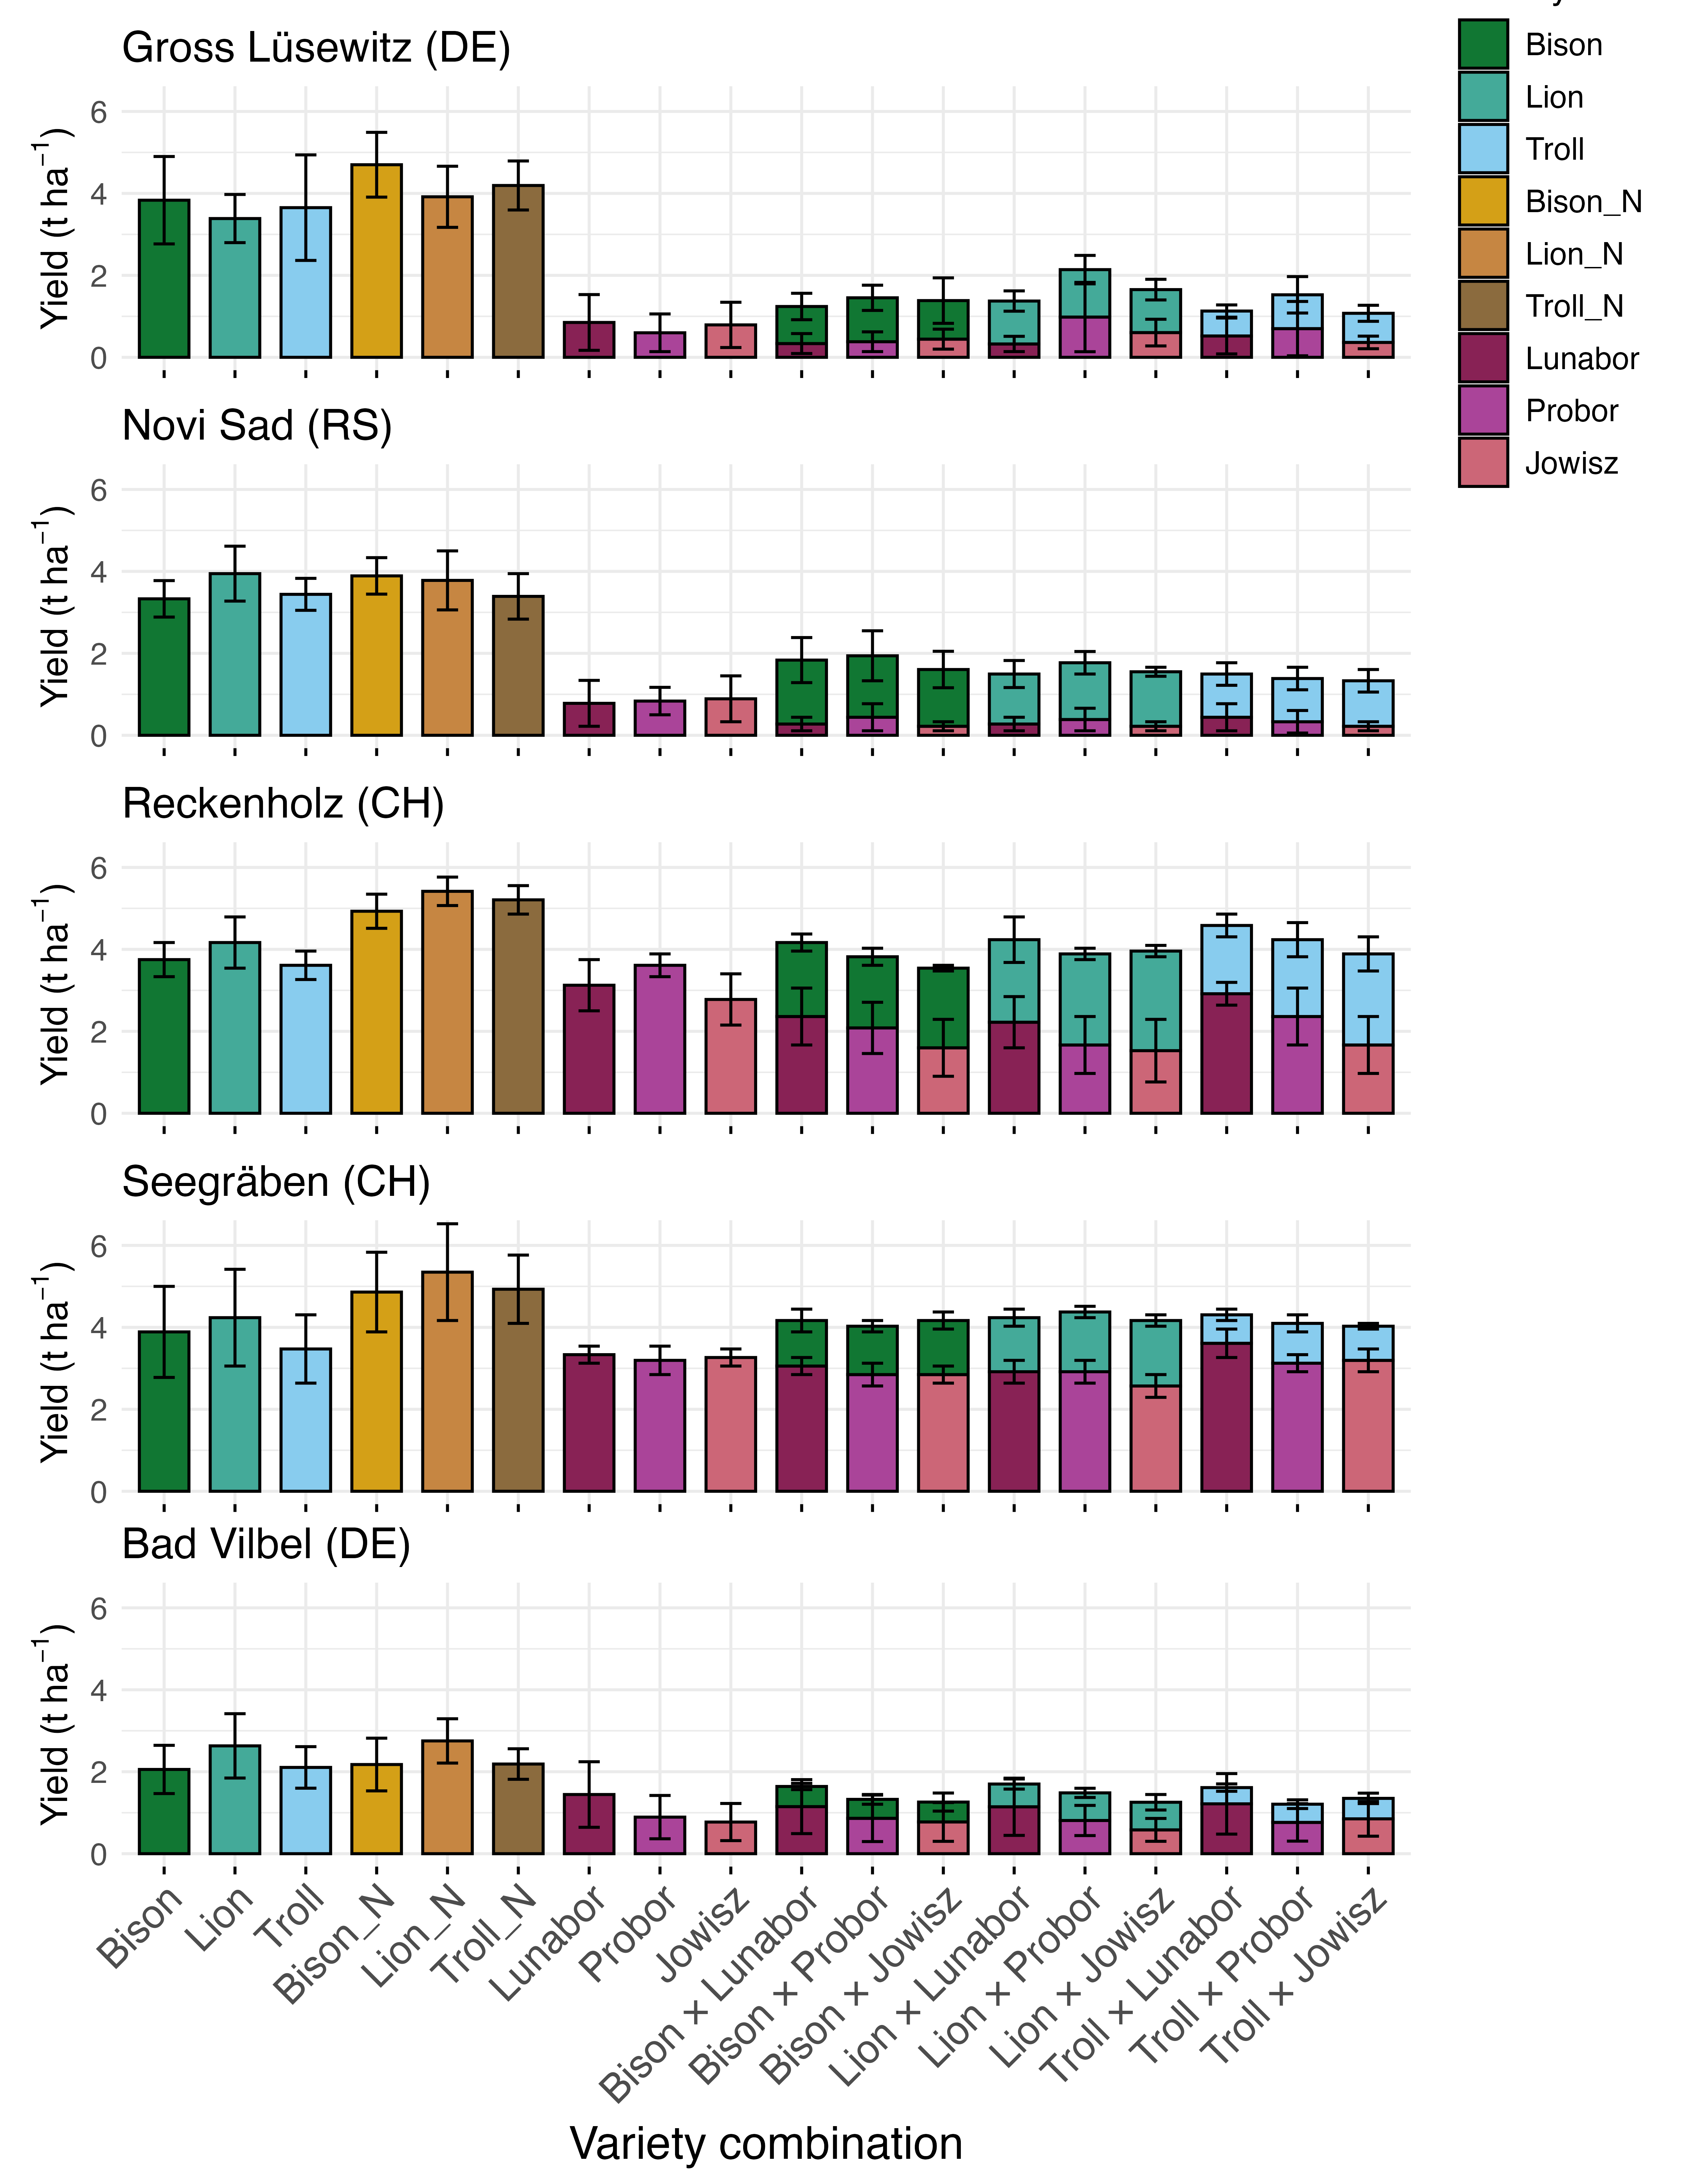
\includegraphics[width=1\linewidth,height=\textheight,keepaspectratio]{./writing/pictures/yieldplot.png}

}

\caption{\label{fig-des}Grain yield overview of pure and mixed stands by
location and the location's country code in brackets. Fertilised oats
are shown in yellow-brown hues. For all graphs, the median value is
represented by the bar height, and the variability (median absolute
deviation) by the error bars. Data were pooled across all years. Bars
with a single colour represent pure stands. In mixed stands, the lower
bar represents the partial lupin values, the upper bar the partial oat
values.}

\end{figure}%

The total yield of Bad Vilbel and Novi Sad were lower across all
observed treatments in the year 2022 than the total yield of Reckenholz,
Seegräben or Gross Lüsewitz (p \textless{} 0.001), whereas in 2023, only
the total yield of Gross Lüsewitz was significantly lower than the yield
recorded in Novi Sad, Reckenholz and Seegräben (Supplemental materials -
Table S3). Further, the yield of all NLL and oat varieties in pure
stands (p \textless{} 0.001) and the partial yield of Jowisz × Troll in
mixed stands differed significantly (p \textless{} 0.05). Across all
locations the average yield of pure NLL and oat stands were not
significantly different from the average yield across all mixtures.
Regarding the proportion of the partial NLL yield in mixtures, Bad
Vilbel and Seegräben exhibited higher NLL than oat proportions of 62\%
and 59\% across all years, respectively, whereas the proportions of the
NLL yield in mixtures amounted to 35\%, 29\% and 24\% in Gross Lüsewitz,
Novi Sad and Reckenholz, respectively (p \textless{} 0.001). A strong
year effect was apparent, resulting in an elevated proportion of the NLL
yield by 16\% in 2022 and 7\% in 2023 across all mixtures, respectively.
Additionally, an oat-interaction effect was detected, resulting in an
increased NLL proportion by 5\% if the NLL were mixed with Troll, and a
decreased proportion by -4.6\% if the NLL were mixed with Lion. All
locations exhibited strong year-by-year variation of the NLL proportion
(Supplemental materials - Appendix A).

\section{Grain-yield performance}\label{grain-yield-performance}

The LER\_N assessed across all locations with regards to fertilised oats
as pure stands, years and treatments did not differ from unity (LER\_N =
1) on a treatment, nor location level (Supplemental materials - Appendix
A). Additionally, no difference could be detected between any pairs of
mixed stand treatments or locations. Though the LER with regards to
unfertilised oats was higher than the LER\_N, it still did not differ
from unity (LER = 1). The total CPR with regards to fertilised and
unfertilised oats as reference pure stands was elevated above unity (E =
2) for all mixed stands, in absence of any treatment effect, amounting
to an average CPR of 5.3 (p \textless{} 0.001), and CPR\_N = 4.6 (p
\textless{} 0.001), respectively, driven by the high oat CPR
(Supplemental materials - Appendix A). The CPR\_N was significantly
lower than the recorded CPR in all mixed treatments but Troll × Lunabor
and Troll × Jowisz (p \textless{} 0.05). None of the CPR or CPR\_N
values exhibited significant differences between treatments across all
locations and years. Similar to the total CPR, the CPR\_oat was above
unity (E = 1), with regards to both the fertilised (CPR\_oat\_N) and the
unfertilised (CPR\_oat) oats as pure reference stands (p \textless{}
0.001). The CPR\_oat was significantly larger than the CPR\_oat\_N for
all mixed Bison and Lion treatments (p \textless{} 0.05), whereas the
mixed Troll treatments were agnostic to the fertilisation regime of
their pure reference stands. Post-hoc comparisons unveiled significantly
higher CPR\_oat and CPR\_oat\_N in three cases of Lion, compared with
Troll, where Lion had shown a CPR exceeding the Trolls CPR by 0.8 - 0.9
(p \textless{} 0.01). However, these effects were restricted to specific
mixed cropping comparisons (e.g.~Lion × Probor compared with Troll ×
Probor) but did not hold true globally for both oat varieties across all
paired mixtures. Conversely to the CPR of oats and the total CPR, the
CPR of NLLs did not differ from unity (E = 1), and there was no effect
of variety, location or year effects.

\section{Grain-yield stability}\label{grain-yield-stability}

\subsection{Static grain-yield
stability}\label{static-grain-yield-stability-1}

The static grain-yield stability, expressed as the coefficient of
variation (CV) calculated on a treatment basis across all
environment-years unveiled no differences in the coefficient of
variation across partial NLL, oat yield or the total yield (Table 3).
However, trends were visible for the yield variation compared with the
treatments' mean yield, the variations was larger in pure stands of NLLs
and some mixed stands, relative to the majority of the mixed stands and
pure (un-)fertilised oat stands. Further, fertilised and unfertilised
oats did not differ significantly with regards to their CV.

\begin{table}

\caption{\label{tbl-overview}}

\centering{

Overview of all grain-yield stability metrics summarised across all
locations on a treatment basis. CV = Coefficient of variation, \(b_{1}\)
= Finlay--Wilkinson slope, \(S^2_{di}\) = Eberhart--Russell deviation
variance, WAAS = weighted average of absolute scores. Letters correspond
to the significance grouping of the pair-wise post-hoc tests (p
\textless{} 0.05) adapted for multiple testing. Variety\_N represents
fertilised pure oat stands.

}

\end{table}%

\begin{longtable}[]{@{}
  >{\raggedleft\arraybackslash}p{(\linewidth - 8\tabcolsep) * \real{0.1889}}
  >{\raggedleft\arraybackslash}p{(\linewidth - 8\tabcolsep) * \real{0.2111}}
  >{\raggedleft\arraybackslash}p{(\linewidth - 8\tabcolsep) * \real{0.2111}}
  >{\raggedleft\arraybackslash}p{(\linewidth - 8\tabcolsep) * \real{0.2000}}
  >{\raggedleft\arraybackslash}p{(\linewidth - 8\tabcolsep) * \real{0.1889}}@{}}
\toprule\noalign{}
\begin{minipage}[b]{\linewidth}\raggedleft
Treatment
\end{minipage} & \begin{minipage}[b]{\linewidth}\raggedleft
CV total yield (not significant)
\end{minipage} & \begin{minipage}[b]{\linewidth}\raggedleft
\(b_{1}\) (responsiveness)
\end{minipage} & \begin{minipage}[b]{\linewidth}\raggedleft
\(S^2_{di}\) (dispersion)
\end{minipage} & \begin{minipage}[b]{\linewidth}\raggedleft
WAAS (sensitivity)
\end{minipage} \\
\midrule\noalign{}
\endhead
\bottomrule\noalign{}
\endlastfoot
Bison & 17 & 0.68a & 0.24a & 0.66a \\
Lion & 16 & 0.63a & 0.14a & 0.58a \\
Troll & 17 & 0.57a & 0.3 a & 0.80a \\
Bison\_N & 18 & 1.1 a & 0.21a & 0.35a \\
Lion\_N & 16 & 1.14b & 0.05b & 0.08b \\
Troll\_N & 15 & 1.2 a & 0.09a & 0.15b \\
Lunabor & 31 & 0.95a & 0.22a & 0.44a \\
Probor & 35 & 1.05a & 0.23a & 0.48a \\
Jowisz & 27 & 1.01a & 0.19a & 0.38a \\
Bison × Lunabor & 17 & 1.08b & 0.004b & 0.11b \\
Bison × Probor & 18 & 0.98c & 0.03b & 0.04b \\
Bison × Jowisz & 18 & 0.91c & 0.06 b & 0.08b \\
Lion × Lunabor & 15 & 1.05b & 0.03 b & 0.21b \\
Lion × Probor & 16 & 1.14a & 0.09 a & 0.34a \\
Lion × Jowisz & 15 & 1.05b & 0.01 b & 0.1b \\
Troll × Lunabor & 17 & 1.21b & 0.03 b & 0.2b \\
Troll × Probor & 27 & 1.23b & 0.06 b & 0.35a \\
Troll × Jowisz & 24 & 1.03b & 0.0005b & 0.067b \\
\end{longtable}

\subsection{Dynamic grain-yield
stability}\label{dynamic-grain-yield-stability-1}

The Finlay-Wilkinson regression coefficients (\(b_{1}\)) measuring the
responsiveness of the total yield to environmental impact was
significantly elevated (\(b_{1}\) \textgreater{} 1) in pure stands of
fertilised Lion, and the mixed stands of Bison × Lunabor, Lion ×
Lunabor, Lion × Jowisz and Troll × Probor, whereas Bison × Probor and
Bison × Jowisz exhibited a buffering capacity (\(b_{1}\) \textless{} 1)
to the environmental influence (p \textless{} 0.005). All pure stands of
NLLs and oats, other than fertilised Lion, and the mixed stands of Lion
× Probor and Troll × Jowisz exhibited average environmental
responsiveness. The Eberhart--Russell deviation variance \(S^2_{di}\)
was highest in pure stands of NLLs, and lowest in mixed treatments
(Table 3). The pure stand of fertilised Lion and Lion × Probor both
combined high responsiveness \(b_{1}\) with low \(S^2_{di}\) dispersion,
indicating that both treatments reliably and consistently respond to
their environmental conditions.

The AMMI model unveiled two groups according to the WAAS-scores: the
sensitivity to environmental conditions of pure unfertilised oat stands
was higher than that of mixed stands (Figure 2, Table 3), further the
AMMI-Model unveiled significant location and treatment effects but no
interaction thereof (Supplemental materials - Table S4). The WAAS-scores
indicated the mixture's higher stabilities across all environment-years,
due to their weaker sensitivity to the location effect. The WAAS scores
also indicated a tendency towards greater stability in fertilised pure
oat stands than in unfertilised pure oat stands, although this
difference was not statistically significant. Across the assessed
interaction principal components axes (IPCAs), IPCA1 distinguished
between the two groups of locations Novi Sad and Gross Lüsewitz
(negative loadings) versus Bad Vilbel, Reckenholz and Seegräben
(positive loadings) (Figure 3). Additionally, IPCA1 clearly
distinguished the pure stands of NLLs (positive loadings) from the oats
(negative loadings). By contrast, IPCA2 distinguished the fertilised
pure stands of oats (negative loadings) from the unfertilised pure
stands of oats. With regards to the factor loading of IPC1 and IPC2, the
two mixtures Lion × Jowisz and Troll × Jowisz plotted closest to the
origin (0,0). These two treatments interacted least with the locations
along IPCA1 and IPCA2, and were thus exhibiting a more stable
performance across all five locations than treatments positioned at
higher Euclidean distance to the origin (Supplemental materials - Table
S4).

\begin{figure}

\centering{

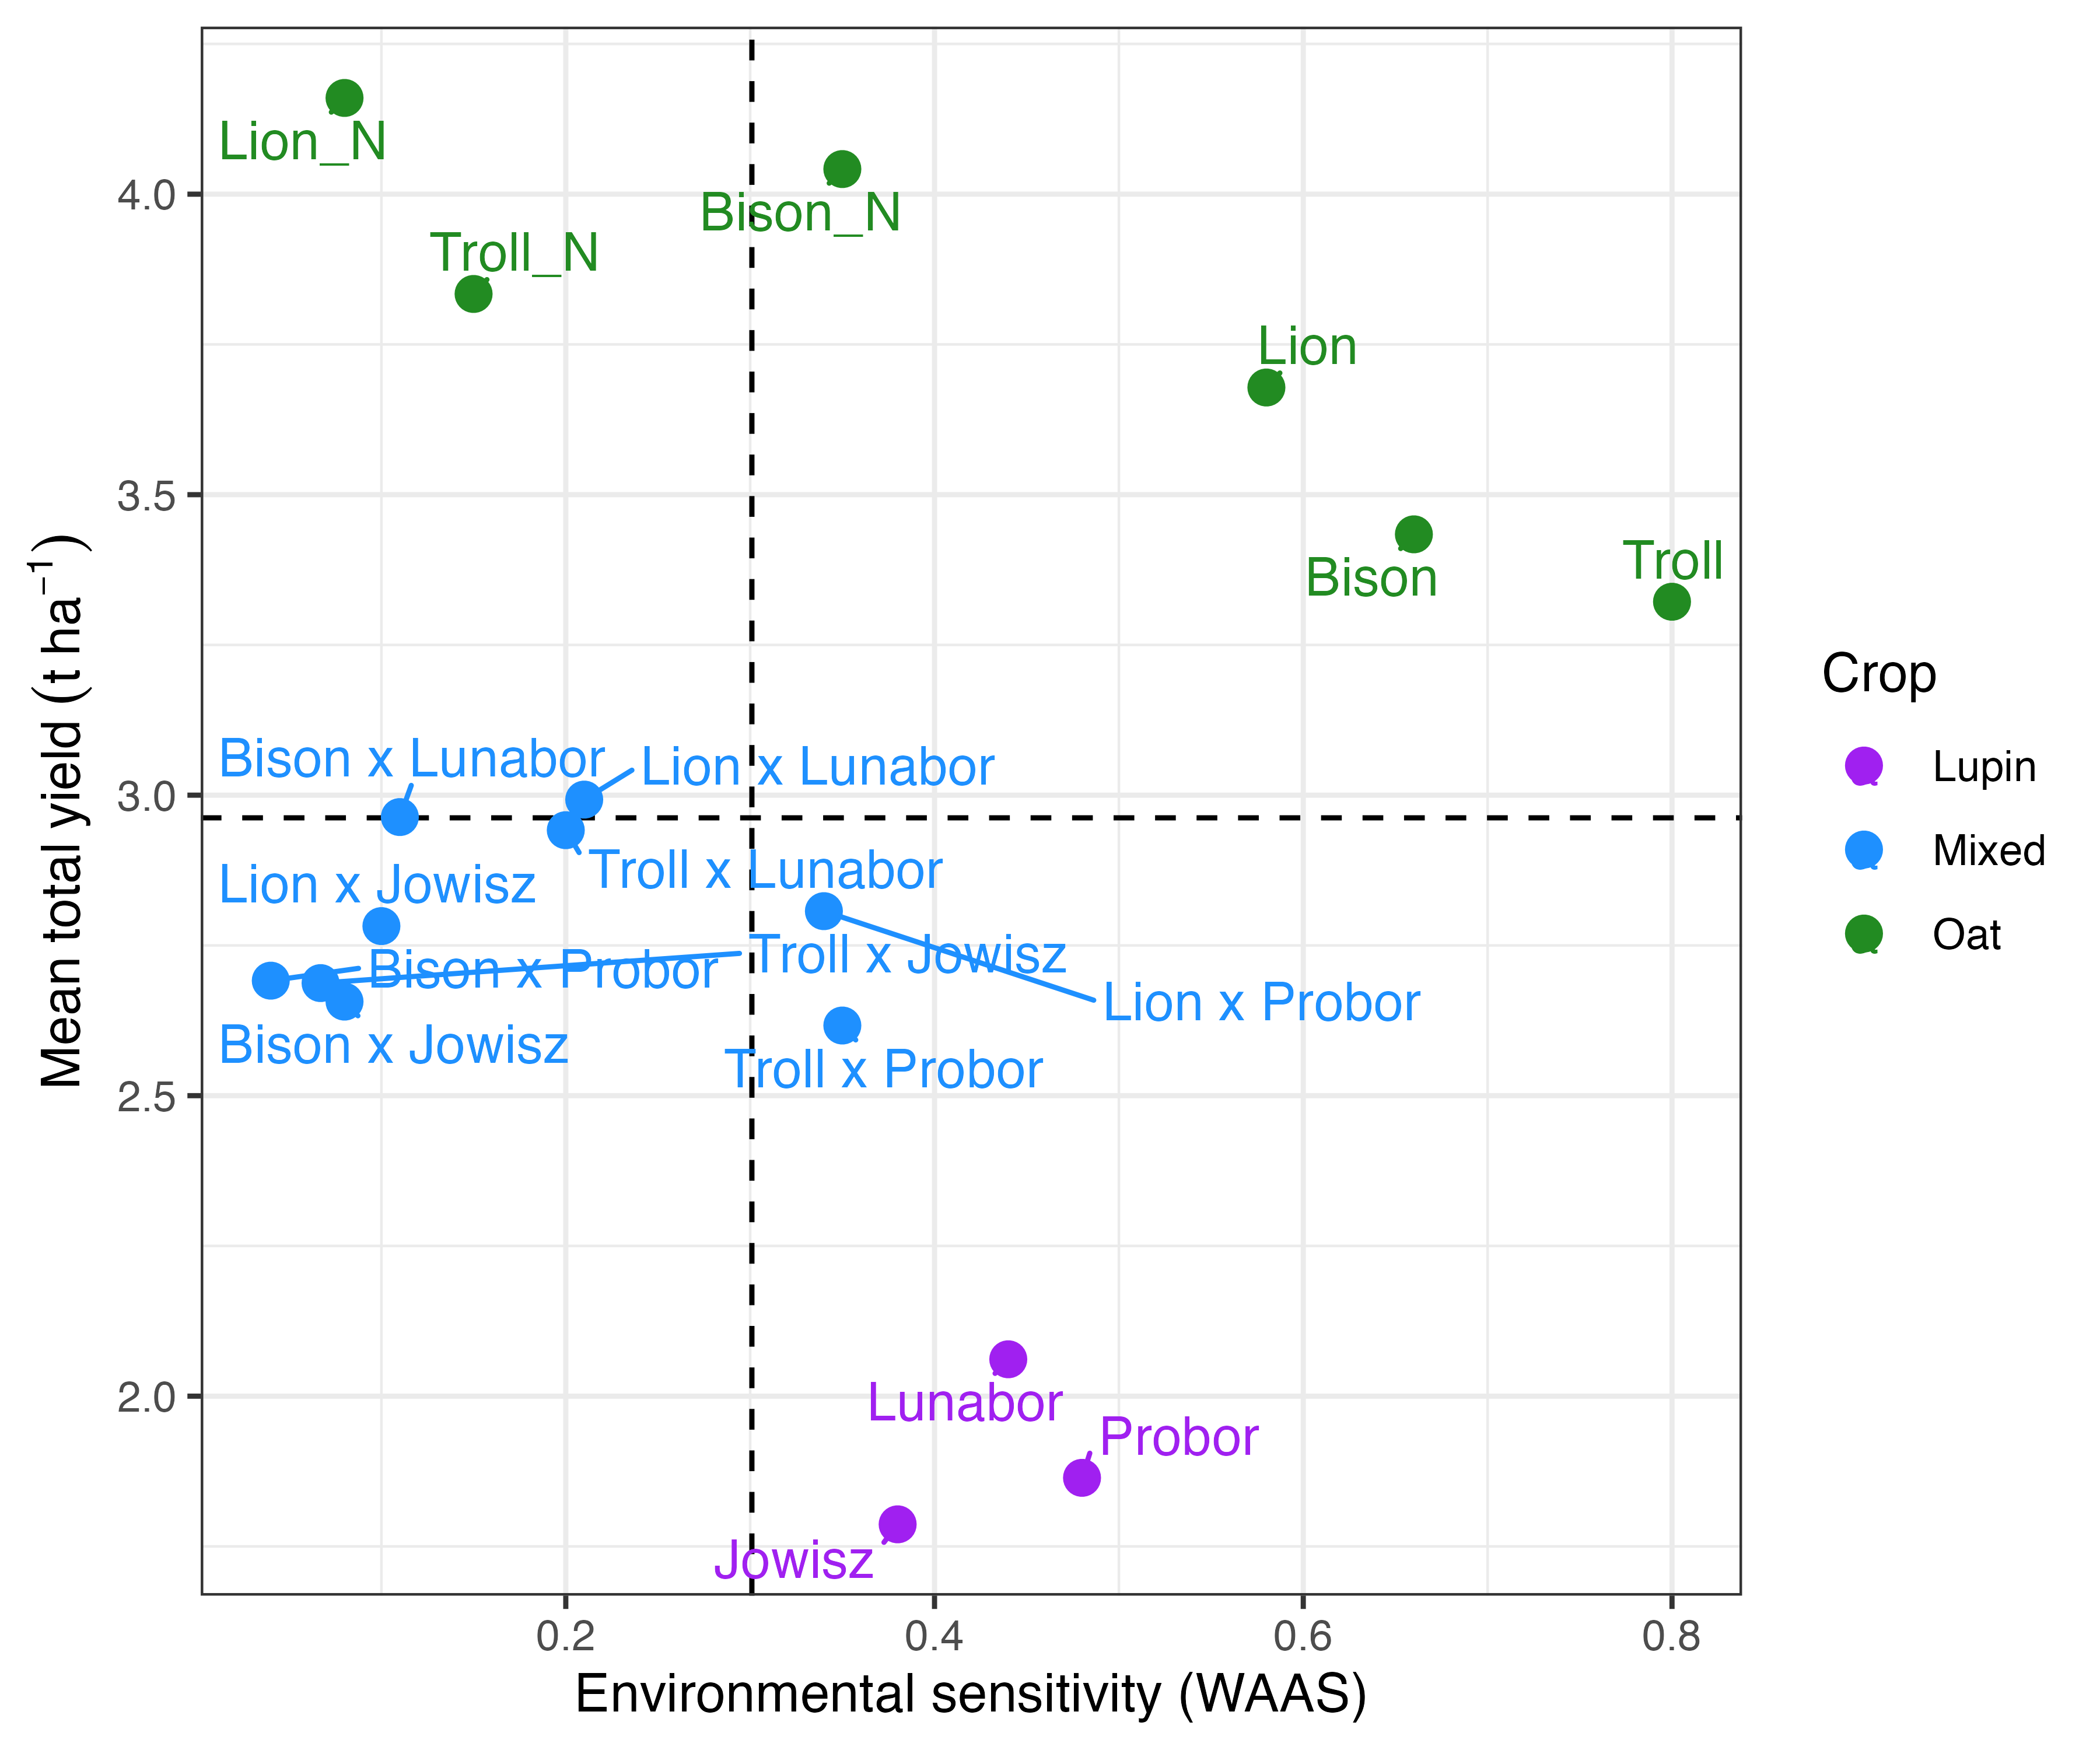
\includegraphics[width=1\linewidth,height=\textheight,keepaspectratio]{./writing/pictures/yieldxwaas.png}

}

\caption{\label{fig-des}Mean total yield plotted against WAAS, an index
of environmental sensitivity, for pure and mixed stands across
2022--2024 (2022--2023 for the Swiss sites). Treatments in the upper
left quadrant combine high yield with low sensitivity, whereas points
further to the right indicate lower grain-yield stability. Dashed lines
mark the median values of both axes.}

\end{figure}%

\begin{figure}

\centering{

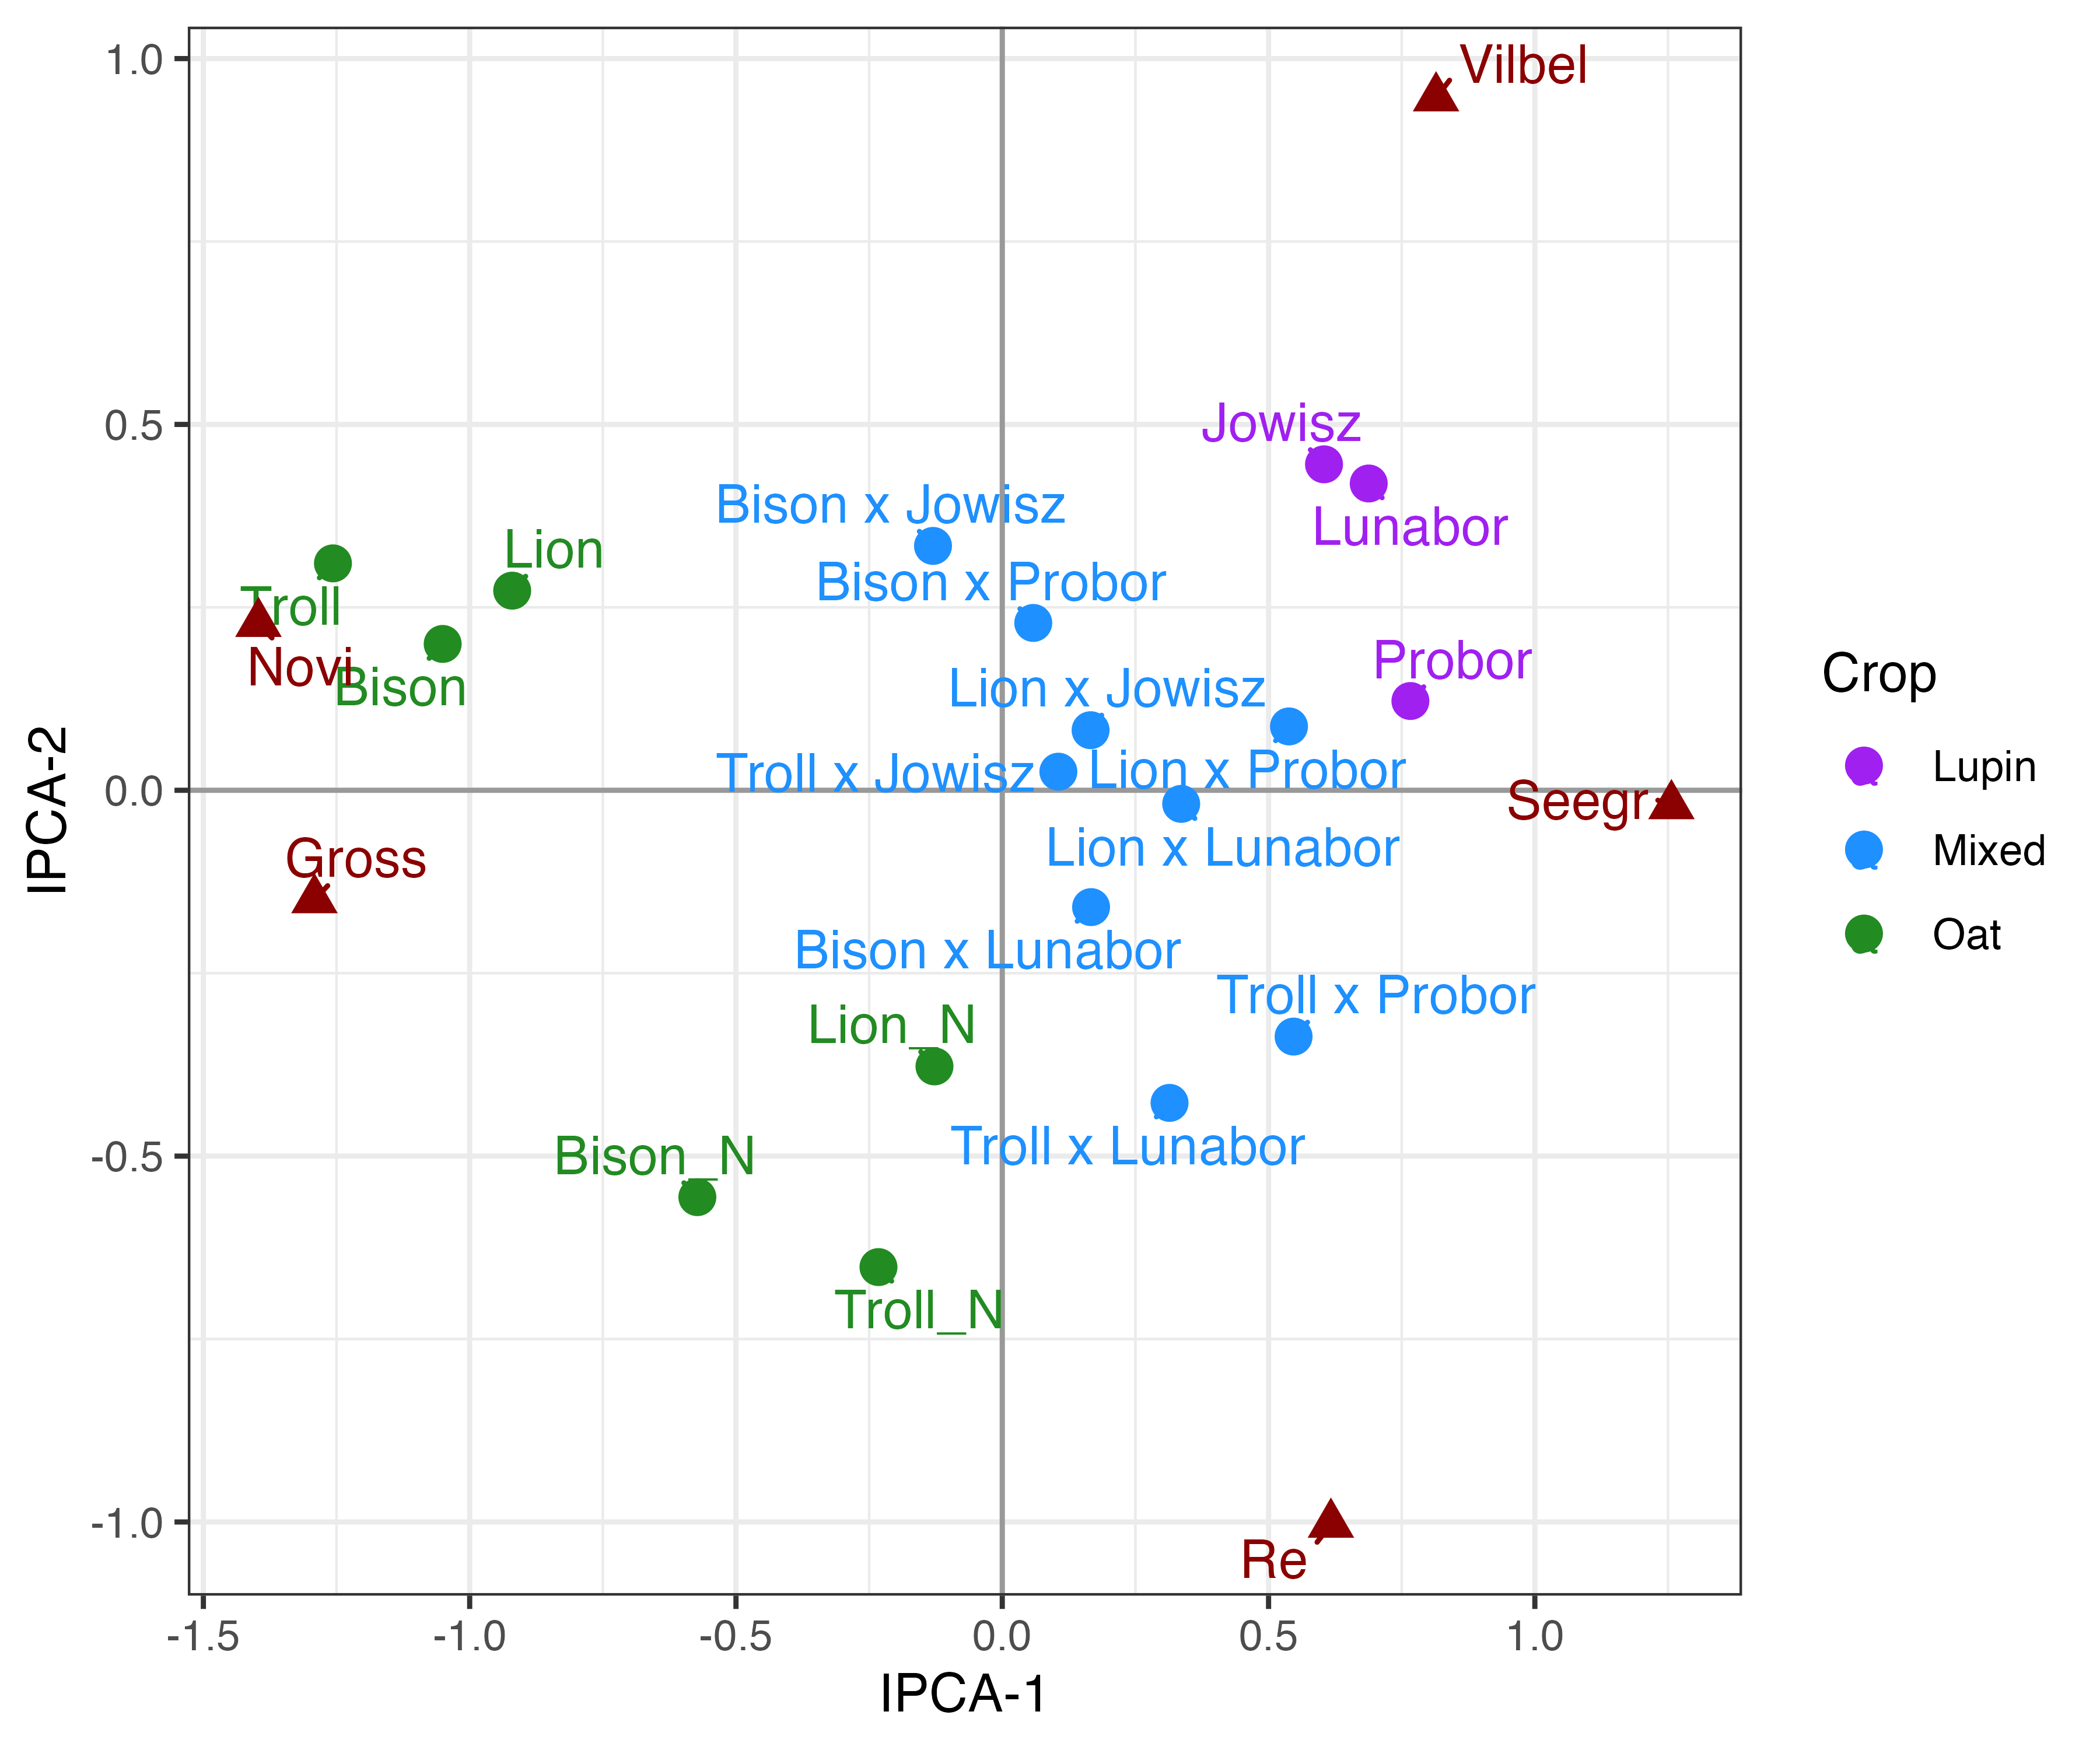
\includegraphics[width=1\linewidth,height=\textheight,keepaspectratio]{./writing/pictures/ammibiplot.png}

}

\caption{\label{fig-des}The additive main effects and multiplicative
interaction (AMMI) biplot of the treatment (circles) and location
(triangles) scores on the first two interaction principal component axes
for total grain yield in pure and mixed stands. The closer a treatment
is positioned to the origin (x,y = 0, 0), the higher was its grain-yield
stability. The following location acronyms were used: Gross - Gross
Lüsewitz (2022 - 2024), Novi- Novi Sad (2022 - 2024), Vilbel - Bad
Vilbel (2022 - 2024), Re - Reckenholz (2022 - 2023) and Seegr -
Seegräben (2022 - 2023).}

\end{figure}%

\chapter{Discussion}\label{discussion}

The multi‑environment evaluation of NLL\,×\,oat mixed cropping
demonstrated that total NLL grain yield was maintained across five
European locations, while several metrics showed an improved temporal
and spatial grain-yield stability relative to the pure stands. The
yields recorded in the present study were broadly within the range
reported for other European pulse × cereal mixed-cropping systems,
although direct comparisons should be interpreted with caution because
the species combinations, environments, and management conditions
differed between studies. For oat-based intercrops, mean yields of
around 3.1 t·ha\textsuperscript{-1} have been reported for oat-vetch
systems in Germany and Sweden and for oat-pea systems in Germany, which
is comparable to the yield range observed at Reckenholz and Seegräben in
the present study (Engbersen et al., 2021; Munz et al., 2025). By
contrast, the remaining locations showed lower total yields across both
pure and mixed stands, consistent with the yield levels reported by Wang
et al. (2012) for lentil-oat intercrops under temperate European
conditions. Because these lower yields occurred consistently across all
pure and mixed treatments within the respective locations, they are more
plausibly attributed to environmental than to varietal effects, in line
with Brooker et al. (2024) showing that intercrop performance remained
strongly modulated by rainfall and crop management. Overall, the yield
levels observed in the present study are in good agreement with the
broader European synthesis by Bedoussac et al. (2015), who reported a
mean intercrop grain yield of 3.3 t·ha\textsuperscript{-1} across 58
pulse × cereal mixtures.

The productivity indices allow for a clear distinction between land use
efficiency and crop performance: The LER did not differ significantly
from unity, but this should not be interpreted as an absence of
mixed-cropping benefit. Rather, it indicates that, on a land-area basis,
the mixtures on average matched the reference pure stands, while the
component responses within the mixtures were asymmetric: This asymmetry
was captured by the CPR: oat CPR and total CPR were consistently above
unity, whereas the CPR of the NLL remained unchanged, showing that the
oat crop captured additional resources without depressing the NLL
performance. This interpretation is consistent with Zustovi et al.
(2024), who showed that mixed cropping indices evaluate different facets
of performance and respond differently to crop ratio and total sowing
density. Accordingly, in a pulse-centric replacement design such as the
present one, the CPR, an indicator accounting for sowing proportion, is
more sensitive than the LER to gains of the minority component.

In the present study, yield maintenance was achieved through a flexible
contribution of the two partners rather than through a fixed proportion:
the NLL proportion in mixture ranged from 24\% in Reckenholz to 62\% in
Bad Vilbel. Similar shifts in pulse × cereal contribution as a function
of weather and location conditions have been reported for oat-vetch
mixtures, underlining that the agronomic value of intercropping lies in
partner compensation across environments rather than in a constant
botanical composition (Bedoussac et al., 2015; Brooker et al., 2024;
Pużyńska et al., 2021). This beneficial effect of mixed cropping in
stabilising the grain yield can be explained by niche c@omplementarity
and mutual yield buffering; the NLL and oat captured resources not used
by the companion crop, thus increasing resource use efficiency, as
supported by recent theoretical work that niche complementarity
underlies mixture advantages (Demie et al., 2022; Hauggaard-Nielsen et
al., 2001; Jensen, 1996). Additionally, in the pulse-centric NLL × oat
mixed cropping system, a strong buffering capacity has been reported,
where the respective yields of NLL and oat are correlated negatively,
thus jointly buffering yield fluctuations compared to pure stands
(Schlup et al., 2026). This pronounced niche complementarity effect in
oat, as reflected by its elevated CPR, coupled to the yield buffering of
both species thus explains the improved grain-yield stability of the
mixtures across all environment-years and their lower response to
environmental stress or stimuli.

Using either fertilised or unfertilised oat pure stands as the reference
for LER led to the same conclusion: LER did not differ between
baselines. This insensitivity to the fertiliser regime is reflected by
substantial spatiotemporal variance in yield across all
environment-years and the low sowing proportion of oat in the mixtures,
which diminishes the weight of the oat component in the summed LER, thus
limiting statistical power. Different mixed cropping indices respond
differently to crop ratio and total sowing density (Zustovi et al.,
2024), eplicitly LER did not elucidate a fertiliser effect, whereas the
CPR did: Both the total CPR and oat‑specific CPR were higher when
mixtures were benchmarked against unfertilised oat stands, rather than
fertilised oat stands, revealing a fertiliser‑mediated gain in the
performance of pure oat stands. Because CPR explicitly scales yields by
the sowing proportion of each species, it provides a
proportion‑corrected measure and is therefore more sensitive to
management effects under imbalanced mixtures than the LER. These
findings are consistent with the prior report of Baxevanos et al. (2020)
that using unfertilised pure stands as references can yield larger
estimates of mixed cropping advantage than using fertilised references.

While the static metric (CV) did not detect significant differences in
grain‑yield stability, the two dynamic approaches, the Finlay-Wilkinson
slope (\(b_{1}\)) and the WAAS, revealed clear contrasts among
treatments. In pure stands, fertilised oat Lion combined an
above‑average responsiveness to environments (slope \(b_{1} > 1\)) with
low dispersion around the regression, indicating a predictable response
in both favourable and unfavourable conditions. Fertilisation enhanced
the stability of oats in pure stands: in the present study, fertilised
Lion and Troll showed significantly higher grain-yield stability
(smaller WAAS-scores) than their unfertilised counterparts, consistent
with the findings of Silva et al.~(2016). Most mixed stands exhibited
elevated responsiveness to the environmental conditions (\(b_{1} > 1\)),
while the most stable mixed treatments exhibited average responsiveness
(\(b_{1} \approx 1\)), coupled to low sensitivity to the environmental
conditions WAAS. Such stability in pulse × cereal mixtures is commonly
attributed to differential species responses and complementarity that
buffer environmental variation and reduce \(G \times E\) interaction,
resulting in more stable yield amongst selected combination
(Raseduzzaman and Jensen, 2017). Across all varieties, the LER remained
consistently at its reference level of one, while the oat and total CPR
values were consistently above one, highlighting a global mixed-cropping
effect of said metrics, which is agnostic to variety-pairing. This
reinforces the evidence that the overall mixed-cropping effect outweighs
cultivar-specific effects, as reported for barley-pea mixtures and for
maize in maize-cowpea mixtures (Hauggaard-Nielsen and Jensen, 2001;
Watiki et al., 1993). The pattern of varying grain-yield stability gains
across the investigated mixtures demonstrates that elevated grain-yield
stability was not only a mixed-cropping effect, but was also depended on
the specific pairing of NLL and oat varieties. Comparable
variety-specific differences have been reported in other pulse × cereal
mixed crops, where mixture performance varied with the complementarity
of the respective partners and their response to resource availability
(Weih et al., 2021). Mechanistic work in oat-NLL mixtures further
suggests that such variability arises from differences in temporal
matching of crop traits, including early vigour, competitive ability,
and the timing of resource capture (Engbersen et al., 2021).
Acknowledging the general mixed-cropping advantage in grain-yield
stability and in parallell focussing on variety-specific interactions
and benefits is thus the best way forward to optimise grain-yield
stability in pulse-cereal production.

The increased dynamic grain-yield stability observed for mixed cropping
in this study extends the findings of Weih et al. (2021) by showing that
under a pulse-centric replacement design (NLL × oat), mixture stability
did not only match but surpassed the pure‑crop benchmarks on dynamic
grain-yield stability. Furthermore, this pattern re-affirms the findings
by Raseduzzaman and Jensen (2017), that replacement-designed mixed crops
of cereals and pulses elevate the grain-yield stability across
environments. Notably, the mixtures Bison × Probor and Troll × Jowisz,
emerged as the most stable, even though neither of their corresponding
pure stands ranked among the most stable, underscoring that stability
must be assessed at the mixture level rather than inferred from
respective pure stands. By quantifying stability with complementary
dynamic metrics (Finlay--Wilkinson slope, \(b_{1}\), and WAAS), the
results of this study show that the stability advantage of mixtures is
not confined to balanced designs; it also holds true under replacement
designs that emphasise the NLL component.

\chapter{Conclusion}\label{conclusion}

This study focusses on the grain-yield performance and stability of
pulse × cereal mixed cropping compared with pure stands between
different locations and years. The patterns observed in the present
study demonstrate that optimal variety mixtures improve grain-yield
stability of both NLL and oat while maintaining crop performance and
land use, opening opportunities for tailoring mixtures to
agri-environmental risk profiles. Moreover, the robust yield-stability
advantage of mixtures across environment-years, which differed six‑fold
in seasonal precipitation, suggests that mixed cropping can effectively
buffer against increasing climate variability, aligning with policy aims
to increase the production of plant-based proteins. Hence, strategic
variety pairing within mixed cropping emerges as an expedient lever to
combine high crop yield and maintain land use performance while
improving the production's resilience. These findings strengthen the
evidence base for incorporating cereals into pulse-centric cropping
strategies to enhance resilience under climate uncertainty and mitigate
the pulses' yield instability. Future studies should address additional
aspects of mixed cropping, such as economic viability as well as
processing and quality of harvested grains.

\chapter{CRediT authorship contribution
statement}\label{credit-authorship-contribution-statement}

\textbf{Schlup Yannik}: Conceptualisation, investigation, data assembly,
statistical analysis, methodology, project administration, resources,
software, visualisation, writing, editing. \textbf{Andrea Gallehr,
Kathrin Neubeck, Matthias Heinrich Herrmann, Radivoje Jevtić, Selma
Schurack, Vesna Župunski}: Conceptualisation, investigation, data
assembly, project administration, resources, review and editing.
\textbf{Lukas Graz}: Statistical analysis, software, visualisation,
review. \textbf{Johan Six}: Review and editing. \textbf{Susanne
Vogelgsang}: Conceptualisation, funding acquisition, methodology,
project administration, resources, review and editing.

\chapter{Funding}\label{funding}

This project was carried out within the Horizon 2020 funded project
CROPDIVA (ID: 101000847). We gratefully acknowledge the financial
support that made this study possible.

\chapter{Declaration of competing
interest}\label{declaration-of-competing-interest}

The authors declare that they have no known personal relationships or
competing financial interests that could have influenced the work
reported in this paper.

\chapter{Declaration of generative AI and AI-assisted technologies in
the writing
process.}\label{declaration-of-generative-ai-and-ai-assisted-technologies-in-the-writing-process.}

During the preparation of this work the authors used GPT-4 (OpenAI,
California, USA) to improve the structure and efficiency of the code to
produce figures and GPT-o3pro (OpenAI, California, USA) in support of
writing the abstract, introduction and discussion. After using this
tool/service, the authors reviewed and edited the content as needed and
take full responsibility for the created content.

\chapter{Data and analytical code}\label{data-and-analytical-code}

The data and code supporting the findings of this study are available at
the project's GitHub repository
(https://github.com/incorey/lupin-oat-grain-yield-stability) and are
permanently archived on Zenodo under DOI
https://doi.org/10.5281/zenodo.XXXXXXX; all materials are released under
the MIT License.

\chapter{Acknowledgments}\label{acknowledgments}

We gratefully acknowledge the field technicians for their invaluable
expertise in the cultivation of NLLs and oats as well as the interns and
MSc students for their assistance in the field and laboratory work.

\chapter{Supplemental materials}\label{supplemental-materials}

Formula 1 - Eberhard-Russell regression for plot-level data \[
Y_{ij} = \mu_i + b_1i\, I_j + \delta_{ij} + \varepsilon_{ij} \tag{1}
\]

Where:

\(Y_{ij}\) is the observed yield of the \(i^{th}\) treatment in the
\(j^{th}\) environment,

\(\mu_i\) is the mean yield of the \(i^{th}\) treatment across all
environments,

\(b_{1i}\) is the Finlay-Wilkinson regression coefficient representing
treatment \(i\)'s responsiveness to the environments,

\(I_j\) is the environmental index, calculated as the mean yield of
environment \(j\) minus the grand mean across environments,

\(\delta_{ij}\)\hspace{0pt}~is~the~deviation~from~the~linear~response~in~environment~\(j\)
used~to~compute~the~deviation~variance~\(S^2_{di}\), and

\(\varepsilon_{ij}\) is the residual term.

Formula 2 - Eberhart-Russell deviation variance

\[
S^2_{di} = \frac{\sum_{j=1}^{E} \delta_{ij}^{\,2}}{E - 2} \tag{2}
\]

Where:

\(\delta_{ij} = Y_{ij} - (\mu_i + b_{1i}I_j)\) are the deviations from
the regression line and

\(E\) are the number of environments.

\begin{table}

\caption{\label{tbl-sites}}

\centering{

Table S1: Field characteristics and husbandry measures per location and
year (environment-year).

}

\end{table}%

\begin{longtable}[]{@{}
  >{\raggedright\arraybackslash}p{(\linewidth - 22\tabcolsep) * \real{0.0931}}
  >{\raggedright\arraybackslash}p{(\linewidth - 22\tabcolsep) * \real{0.0637}}
  >{\raggedright\arraybackslash}p{(\linewidth - 22\tabcolsep) * \real{0.0686}}
  >{\raggedright\arraybackslash}p{(\linewidth - 22\tabcolsep) * \real{0.0637}}
  >{\raggedright\arraybackslash}p{(\linewidth - 22\tabcolsep) * \real{0.0931}}
  >{\raggedright\arraybackslash}p{(\linewidth - 22\tabcolsep) * \real{0.0686}}
  >{\raggedright\arraybackslash}p{(\linewidth - 22\tabcolsep) * \real{0.1078}}
  >{\raggedright\arraybackslash}p{(\linewidth - 22\tabcolsep) * \real{0.1078}}
  >{\raggedright\arraybackslash}p{(\linewidth - 22\tabcolsep) * \real{0.1275}}
  >{\raggedright\arraybackslash}p{(\linewidth - 22\tabcolsep) * \real{0.0882}}
  >{\raggedright\arraybackslash}p{(\linewidth - 22\tabcolsep) * \real{0.0539}}
  >{\raggedright\arraybackslash}p{(\linewidth - 22\tabcolsep) * \real{0.0637}}@{}}
\toprule\noalign{}
\begin{minipage}[b]{\linewidth}\raggedright
Location and year
\end{minipage} & \begin{minipage}[b]{\linewidth}\raggedright
Latitude (°N)
\end{minipage} & \begin{minipage}[b]{\linewidth}\raggedright
Longitude (°E)
\end{minipage} & \begin{minipage}[b]{\linewidth}\raggedright
Pre-crop
\end{minipage} & \begin{minipage}[b]{\linewidth}\raggedright
Pre-pre-crop
\end{minipage} & \begin{minipage}[b]{\linewidth}\raggedright
Sowing
\end{minipage} & \begin{minipage}[b]{\linewidth}\raggedright
Weeding 1
\end{minipage} & \begin{minipage}[b]{\linewidth}\raggedright
Weeding 2
\end{minipage} & \begin{minipage}[b]{\linewidth}\raggedright
Oat fertilisation (kgNha\textsuperscript{-1})
\end{minipage} & \begin{minipage}[b]{\linewidth}\raggedright
Pest intervention
\end{minipage} & \begin{minipage}[b]{\linewidth}\raggedright
Harvest
\end{minipage} & \begin{minipage}[b]{\linewidth}\raggedright
Soil-type
\end{minipage} \\
\midrule\noalign{}
\endhead
\bottomrule\noalign{}
\endlastfoot
Bad Vilbel 2022 & 50.2 & 8.6 & - & - & March 29 & April 28 & May 5 & 43
& - & July 14 & Sandy loam \\
Bad Vilbel 2023 & 50.2 & 8.8 & - & - & April 06 & - & - & 40 & - &
August 1 & Sandy loam \\
Bad Vilbel 2024 & 50.2 & 8.7 & - & - & April 24 & - & - & 35 & - & July
29 & Sandy loam \\
Gross Lüsewitz 2022 & 54.1 & 13.3 & Lupin & Lolium & March 31 & April 5
(Stomp Aqua) & & 40 & - & August 17 & Sandy loam \\
Gross Lüsewitz 2023 & 54.1 & 13.3 & Lupin & Lolium & April 5 & - & & 40
& - & August 22 & Sandy loam \\
Gross Lüsewitz 2024 & 54.1 & 13.3 & Lolium & Winter rye & March 22 &
March 27 (Stomp Aqua) & & 40 & - & August 8 & Sandy loam \\
Novi Sad 2023 & 45.3 & 19.8 & Maize & Winter wheat & May 5 & manual &
manual & 60 & Vantex 60CS against Oulema ssp. & July 28 & Loamy
chernozem \\
Novi Sad 2024 & 45.3 & 19.8 & Soybean & Maize & March 30 & manual &
manual & 60 & Vantex 60CS against Oulema ssp. & July 19 & Loamy
chernozem \\
Novi Sad 2025 & 45.3 & 19.8 & Soybean & Maize & February 28 & manual &
manual & 60 & Vantex 60CS against Oulema ssp. & July 1 & Loamy
chernozem \\
Reckenholz 2022 & 47.4 & 8.5 & Silage maize & Flower strip & March 4 &
March 21 (mechanical) & April 5 (mechanical) & 27.5 & - & July 12 &
Loamy clay \\
Reckenholz 2023 & 47.4 & 8.5 & Silage maize & Artificial pasture &
February 16 & February 22 (mechanical) & April 4 (mechanical) & 30 & - &
July 10 & Loamy clay \\
Seegräben 2022 & 47.3 & 8.9 & Silage maize & Winter wheat & March 10 &
March 17 (mechanical) & March 31 (mechanical) & 27.5 & - & July 19 &
Sandy loam \\
Seegräben 2023 & 47.4 & 8.9 & Silage maize & Winter barley & February 22
& March 1 (mechanical) & April 5 (mechanical) & 30 & - & July 19 & Sandy
loam \\
\end{longtable}

\begin{table}

\caption{\label{tbl-mdls}}

\centering{

Table S2: Statistical models deployed to analyse the data. The
characteristics explain the details of the model. Each response variable
(attribute) in the present study was analysed with one or more of the
models listed in the table. To analyse the effect of canopy height
difference onto the narrow-leaved lupin proportion and the total yield,
model M3 was adapted replacing the predictor treatment with canopy
height difference.

}

\end{table}%

\begin{longtable}[]{@{}
  >{\raggedright\arraybackslash}p{(\linewidth - 2\tabcolsep) * \real{0.1695}}
  >{\raggedright\arraybackslash}p{(\linewidth - 2\tabcolsep) * \real{0.8305}}@{}}
\toprule\noalign{}
\begin{minipage}[b]{\linewidth}\raggedright
Model
\end{minipage} & \begin{minipage}[b]{\linewidth}\raggedright
Characteristics
\end{minipage} \\
\midrule\noalign{}
\endhead
\bottomrule\noalign{}
\endlastfoot
M1 & This model answered if the response variable differed in mixtures
and pure NLLs (or analogously oats) across all varieties. It performed
an ANOVA using the NLL/oat-variety and the binary variable stand =
mixed. This model considered each species separately. \\
M2 & M2 answered if the response variable differed in mixtures and pure
NLLs or oats. Here, this was achieved by computing the linear contrasts
of each pure NLL/oat variety with the mean of its respective mixtures.
This model considered each species separately. \\
M3 & On the subset of only mixed plots, M3 performed a two-way (mixed)
ANOVA with the factors oat variety and NLL variety (adjusting for
location, year, and block). This model considered both species together.
Further, M3 performed post-hoc comparisons of the treatments and
locations. \\
M4 & M4 answered the question, if the estimated value of the treatments
with mixed stands (e.g.~the land equivalent ratio) was significantly
different from an expected value (e.g.~LER = 1) after a Bonferroni
correction (with the respective 12 coefficients). \\
\end{longtable}

\begin{table}

\caption{\label{tbl-yield-locationyear}}

\centering{

Table S3: Year × location median yields and median absolute deviations
(tha\textsuperscript{-1}) aggregated across blocks.

}

\end{table}%

\begin{longtable}[]{@{}
  >{\raggedright\arraybackslash}p{(\linewidth - 26\tabcolsep) * \real{0.0714}}
  >{\raggedright\arraybackslash}p{(\linewidth - 26\tabcolsep) * \real{0.0714}}
  >{\raggedright\arraybackslash}p{(\linewidth - 26\tabcolsep) * \real{0.0714}}
  >{\raggedright\arraybackslash}p{(\linewidth - 26\tabcolsep) * \real{0.0714}}
  >{\raggedright\arraybackslash}p{(\linewidth - 26\tabcolsep) * \real{0.0714}}
  >{\raggedright\arraybackslash}p{(\linewidth - 26\tabcolsep) * \real{0.0714}}
  >{\raggedright\arraybackslash}p{(\linewidth - 26\tabcolsep) * \real{0.0714}}
  >{\raggedright\arraybackslash}p{(\linewidth - 26\tabcolsep) * \real{0.0714}}
  >{\raggedright\arraybackslash}p{(\linewidth - 26\tabcolsep) * \real{0.0714}}
  >{\raggedright\arraybackslash}p{(\linewidth - 26\tabcolsep) * \real{0.0714}}
  >{\raggedright\arraybackslash}p{(\linewidth - 26\tabcolsep) * \real{0.0714}}
  >{\raggedright\arraybackslash}p{(\linewidth - 26\tabcolsep) * \real{0.0714}}
  >{\raggedright\arraybackslash}p{(\linewidth - 26\tabcolsep) * \real{0.0714}}
  >{\raggedright\arraybackslash}p{(\linewidth - 26\tabcolsep) * \real{0.0714}}@{}}
\toprule\noalign{}
\begin{minipage}[b]{\linewidth}\raggedright
Treatment
\end{minipage} & \begin{minipage}[b]{\linewidth}\raggedright
Gross 2022
\end{minipage} & \begin{minipage}[b]{\linewidth}\raggedright
Gross 2023
\end{minipage} & \begin{minipage}[b]{\linewidth}\raggedright
Gross 2024
\end{minipage} & \begin{minipage}[b]{\linewidth}\raggedright
Novi 2022
\end{minipage} & \begin{minipage}[b]{\linewidth}\raggedright
Novi 2023
\end{minipage} & \begin{minipage}[b]{\linewidth}\raggedright
Novi 2024
\end{minipage} & \begin{minipage}[b]{\linewidth}\raggedright
Re 2022
\end{minipage} & \begin{minipage}[b]{\linewidth}\raggedright
Re 2023
\end{minipage} & \begin{minipage}[b]{\linewidth}\raggedright
Seegr 2022
\end{minipage} & \begin{minipage}[b]{\linewidth}\raggedright
Seegr 2023
\end{minipage} & \begin{minipage}[b]{\linewidth}\raggedright
Vilbel 2022
\end{minipage} & \begin{minipage}[b]{\linewidth}\raggedright
Vilbel 2023
\end{minipage} & \begin{minipage}[b]{\linewidth}\raggedright
Vilbel 2024
\end{minipage} \\
\midrule\noalign{}
\endhead
\bottomrule\noalign{}
\endlastfoot
Bison & 3.83 ± 0.01 & 2.30 ± 0.08 & 4.85 ± 0.12 & 2.95 ± 0.22 & 3.33 ±
0.11 & 4.38 ± 0.06 & 4.51 ± 0.69 & 3.33 ± 0.28 & 5.35 ± 0.35 & 3.06 ±
0.21 & 2.81 ± 0.12 & 0.77 ± 0.14 & 1.96 ± 0.19 \\
Lion & 3.39 ± 0.17 & 3.24 ± 0.02 & 4.58 ± 0.15 & 2.95 ± 0.17 & 4.56 ±
0.17 & 4.22 ± 0.22 & 4.93 ± 0.35 & 3.75 ± 0.21 & 5.42 ± 0.07 & 3.13 ±
0.14 & 3.24 ± 0.52 & 1.60 ± 0.00 & 2.70 ± 0.33 \\
Troll & 3.95 ± 0.41 & 2.05 ± 0.15 & 4.75 ± 0.37 & 3.17 ± 0.17 & 3.67 ±
0.50 & 3.73 ± 0.23 & 3.82 ± 0.49 & 3.47 ± 0.14 & 4.79 ± 0.42 & 2.71 ±
0.07 & 2.46 ± 0.34 & 1.22 ± 0.28 & 2.11 ± 0.39 \\
Bison\_N & 4.88 ± 0.31 & 2.52 ± 0.08 & 5.07 ± 0.47 & 3.38 ± 0.34 & 3.55
± 0.34 & 4.33 ± 0.06 & 4.93 ± 0.28 & 4.79 ± 0.42 & 6.04 ± 0.42 & 4.03 ±
0.21 & 3.31 ± 0.13 & 1.33 ± 0.52 & 2.03 ± 0.47 \\
Lion\_N & 4.29 ± 0.25 & 2.60 ± 0.59 & 4.17 ± 0.71 & 2.95 ± 0.11 & 4.55 ±
0.34 & 4.17 ± 0.39 & 5.07 ± 0.63 & 5.69 ± 0.07 & 6.53 ± 0.07 & 4.10 ±
0.14 & 3.02 ± 0.23 & 1.62 ± 0.20 & 2.89 ± 0.67 \\
Troll\_N & 4.27 ± 0.11 & 2.33 ± 0.14 & 4.77 ± 0.08 & 2.83 ± 0.50 & 3.11
± 0.28 & 4.39 ± 0.28 & 5.42 ± 0.28 & 4.86 ± 0.35 & 5.76 ± 0.21 & 4.10 ±
0.21 & 2.50 ± 0.13 & 1.80 ± 0.03 & 2.51 ± 0.04 \\
Lunabor & 2.86 ± 0.15 & 0.22 ± 0.08 & 0.62 ± 0.43 & 0.22 ± 0.00 & 2.50 ±
0.06 & 0.78 ± 0.00 & 3.13 ± 0.14 & 2.22 ± 1.32 & 3.54 ± 0.42 & 3.33 ±
0.07 & 2.44 ± 0.20 & 1.39 ± 0.08 & 0.33 ± 0.15 \\
Probor & 2.25 ± 0.15 & 0.10 ± 0.05 & 0.35 ± 0.14 & 0.39 ± 0.05 & 1.50 ±
0.22 & 0.83 ± 0.16 & 3.61 ± 0.00 & 1.81 ± 1.25 & 3.19 ± 0.21 & 3.33 ±
0.42 & 2.26 ± 0.10 & 0.88 ± 0.12 & 0.43 ± 0.15 \\
Jowisz & 2.47 ± 0.13 & 0.40 ± 0.05 & 0.67 ± 0.46 & 0.28 ± 0.06 & 1.73 ±
0.11 & 0.89 ± 0.22 & 3.26 ± 0.14 & 1.39 ± 0.14 & 3.68 ± 0.14 & 3.19 ±
0.07 & 2.06 ± 0.10 & 1.02 ± 0.07 & 0.38 ± 0.12 \\
Bison × Lunabor & 3.49 ± 0.08 & 0.79 ± 0.33 & 3.18 ± 0.33 & 1.56 ± 0.33
& 2.89 ± 0.17 & 2.33 ± 0.11 & 4.72 ± 0.07 & 3.47 ± 0.56 & 4.31 ± 0.28 &
4.17 ± 0.07 & 2.73 ± 0.07 & 1.47 ± 0.27 & 1.19 ± 0.21 \\
Bison × Probor & 3.16 ± 0.16 & 1.01 ± 0.27 & 2.87 ± 0.30 & 1.61 ± 0.12 &
2.45 ± 0.05 & 2.61 ± 0.11 & 3.82 ± 0.35 & 2.64 ± 0.07 & 4.03 ± 0.00 &
4.03 ± 0.07 & 2.72 ± 0.08 & 1.17 ± 0.08 & 0.70 ± 0.28 \\
Bison × Jowisz & 3.02 ± 0.16 & 0.63 ± 0.00 & 3.44 ± 0.06 & 1.55 ± 0.16 &
2.62 ± 0.17 & 2.38 ± 0.11 & 3.61 ± 0.14 & 2.50 ± 0.35 & 4.51 ± 0.14 &
3.47 ± 0.21 & 2.69 ± 0.09 & 0.88 ± 0.25 & 0.83 ± 0.21 \\
Lion × Lunabor & 3.24 ± 0.18 & 1.21 ± 0.14 & 3.20 ± 0.09 & 1.33 ± 0.00 &
2.95 ± 0.22 & 2.39 ± 0.11 & 4.03 ± 0.35 & 3.96 ± 0.07 & 4.79 ± 0.14 &
3.96 ± 0.07 & 3.11 ± 0.24 & 1.65 ± 0.06 & 1.17 ± 0.36 \\
Lion × Probor & 2.90 ± 0.05 & 0.90 ± 0.15 & 1.22 ± 0.00 & 1.50 ± 0.05 &
2.55 ± 0.17 & 2.39 ± 0.17 & 4.17 ± 0.14 & 3.19 ± 0.56 & 4.17 ± 0.00 &
4.10 ± 0.28 & 2.69 ± 0.12 & 1.47 ± 0.20 & 1.28 ± 0.28 \\
Lion × Jowisz & 3.08 ± 0.12 & 1.09 ± 0.17 & 3.19 ± 0.00 & 1.44 ± 0.00 &
2.94 ± 0.11 & 2.17 ± 0.11 & 4.24 ± 0.21 & 2.99 ± 0.28 & 4.65 ± 0.14 &
3.75 ± 0.07 & 2.73 ± 0.03 & 0.93 ± 0.03 & 1.11 ± 0.37 \\
Troll × Lunabor & 3.22 ± 0.12 & 0.68 ± 0.19 & 3.44 ± 0.45 & 1.17 ± 0.22
& 2.89 ± 0.00 & 2.23 ± 0.00 & 4.51 ± 0.07 & 4.17 ± 0.69 & 4.51 ± 0.21 &
3.96 ± 0.14 & 2.56 ± 0.06 & 1.73 ± 0.02 & 0.95 ± 0.36 \\
Troll × Probor & 3.09 ± 0.15 & 0.43 ± 0.21 & 1.00 ± 0.68 & 1.17 ± 0.06 &
2.06 ± 0.39 & 1.89 ± 0.12 & 4.31 ± 0.14 & 3.54 ± 0.56 & 4.17 ± 0.35 &
3.96 ± 0.14 & 2.50 ± 0.10 & 1.35 ± 0.18 & 0.67 ± 0.11 \\
Troll × Jowisz & 2.74 ± 0.13 & 0.55 ± 0.42 & 3.36 ± 0.41 & 1.22 ± 0.11 &
2.56 ± 0.17 & 2.11 ± 0.16 & 3.68 ± 0.35 & 3.26 ± 0.49 & 4.44 ± 0.07 &
3.47 ± 0.28 & 2.54 ± 0.09 & 1.03 ± 0.18 & 0.87 ± 0.07 \\
\end{longtable}

\begin{table}

\caption{\label{tbl-ammi}}

\centering{

Table S4: The additive main effects and multiplicative interaction
(AMMI) model output

}

\end{table}%

\begin{longtable}[]{@{}
  >{\raggedright\arraybackslash}p{(\linewidth - 26\tabcolsep) * \real{0.0583}}
  >{\raggedright\arraybackslash}p{(\linewidth - 26\tabcolsep) * \real{0.0680}}
  >{\raggedright\arraybackslash}p{(\linewidth - 26\tabcolsep) * \real{0.0485}}
  >{\raggedright\arraybackslash}p{(\linewidth - 26\tabcolsep) * \real{0.0777}}
  >{\raggedright\arraybackslash}p{(\linewidth - 26\tabcolsep) * \real{0.0777}}
  >{\raggedright\arraybackslash}p{(\linewidth - 26\tabcolsep) * \real{0.0777}}
  >{\raggedright\arraybackslash}p{(\linewidth - 26\tabcolsep) * \real{0.0777}}
  >{\raggedright\arraybackslash}p{(\linewidth - 26\tabcolsep) * \real{0.0680}}
  >{\raggedright\arraybackslash}p{(\linewidth - 26\tabcolsep) * \real{0.0777}}
  >{\raggedright\arraybackslash}p{(\linewidth - 26\tabcolsep) * \real{0.0874}}
  >{\raggedright\arraybackslash}p{(\linewidth - 26\tabcolsep) * \real{0.0583}}
  >{\raggedright\arraybackslash}p{(\linewidth - 26\tabcolsep) * \real{0.0680}}
  >{\raggedright\arraybackslash}p{(\linewidth - 26\tabcolsep) * \real{0.0777}}
  >{\raggedright\arraybackslash}p{(\linewidth - 26\tabcolsep) * \real{0.0777}}@{}}
\toprule\noalign{}
\begin{minipage}[b]{\linewidth}\raggedright
Type
\end{minipage} & \begin{minipage}[b]{\linewidth}\raggedright
Code
\end{minipage} & \begin{minipage}[b]{\linewidth}\raggedright
Y
\end{minipage} & \begin{minipage}[b]{\linewidth}\raggedright
PC1
\end{minipage} & \begin{minipage}[b]{\linewidth}\raggedright
PC2
\end{minipage} & \begin{minipage}[b]{\linewidth}\raggedright
PC3
\end{minipage} & \begin{minipage}[b]{\linewidth}\raggedright
PC4
\end{minipage} & \begin{minipage}[b]{\linewidth}\raggedright
WAAS
\end{minipage} & \begin{minipage}[b]{\linewidth}\raggedright
PctResp
\end{minipage} & \begin{minipage}[b]{\linewidth}\raggedright
PctWAAS
\end{minipage} & \begin{minipage}[b]{\linewidth}\raggedright
wRes
\end{minipage} & \begin{minipage}[b]{\linewidth}\raggedright
wWAAS
\end{minipage} & \begin{minipage}[b]{\linewidth}\raggedright
OrResp
\end{minipage} & \begin{minipage}[b]{\linewidth}\raggedright
OrWAAS
\end{minipage} \\
\midrule\noalign{}
\endhead
\bottomrule\noalign{}
\endlastfoot
GEN & 10 & 3.0 & 0.081 & 0.270 & -0.250 & 0.069 & 0.081 & 47.0 & 93.0 &
50 & 50 & 6 & 6 \\
GEN & 11 & 2.9 & -0.081 & -0.390 & 0.014 & 0.030 & 0.081 & 40.0 & 93.0 &
50 & 50 & 9 & 7 \\
GEN & 12 & 2.8 & -0.053 & -0.530 & 0.066 & 0.041 & 0.053 & 36.0 & 97.0 &
50 & 50 & 12 & 3 \\
GEN & 13 & 3.1 & 0.084 & 0.060 & -0.055 & 0.170 & 0.084 & 52.0 & 93.0 &
50 & 50 & 4 & 9 \\
GEN & 14 & 3.0 & 0.083 & -0.140 & 0.0059 & -0.290 & 0.083 & 47.0 & 93.0
& 50 & 50 & 7 & 8 \\
GEN & 15 & 3.0 & -0.063 & -0.230 & -0.110 & -0.059 & 0.063 & 44.0 & 96.0
& 50 & 50 & 8 & 4 \\
GEN & 16 & 3.1 & -0.048 & 0.370 & 0.014 & -0.120 & 0.048 & 49.0 & 98.0 &
50 & 50 & 5 & 2 \\
GEN & 17 & 2.8 & 0.080 & 0.370 & -0.230 & -0.150 & 0.080 & 38.0 & 94.0 &
50 & 50 & 11 & 5 \\
GEN & 18 & 2.8 & -0.032 & -0.120 & -0.075 & 0.061 & 0.032 & 39.0 & 100.0
& 50 & 50 & 10 & 1 \\
GEN & 4 & 4.3 & -0.760 & -0.0005 & -0.320 & 0.200 & 0.760 & 95.0 & 0.0 &
50 & 50 & 2 & 15 \\
GEN & 5 & 4.4 & -0.480 & 0.019 & 0.510 & -0.0085 & 0.480 & 100.0 & 38.0
& 50 & 50 & 1 & 10 \\
GEN & 6 & 4.0 & -0.490 & 0.260 & 0.190 & -0.120 & 0.490 & 85.0 & 37.0 &
50 & 50 & 3 & 11 \\
GEN & 7 & 2.1 & 0.580 & -0.035 & 0.072 & 0.250 & 0.580 & 12.0 & 26.0 &
50 & 50 & 13 & 14 \\
GEN & 8 & 1.9 & 0.560 & 0.300 & 0.260 & 0.150 & 0.560 & 4.0 & 28.0 & 50
& 50 & 14 & 13 \\
GEN & 9 & 1.8 & 0.550 & -0.210 & -0.097 & -0.240 & 0.550 & 0.0 & 29.0 &
50 & 50 & 15 & 12 \\
ENV & Gross & 2.7 & -0.600 & -0.110 & -0.600 & 0.120 & 0.600 & 43.0 &
41.0 & 50 & 50 & 3 & 3 \\
ENV & Novi & 2.5 & -0.740 & -0.370 & 0.500 & 0.058 & 0.740 & 33.0 & 26.0
& 50 & 50 & 4 & 4 \\
ENV & Re & 3.9 & -0.058 & 0.910 & 0.120 & -0.015 & 0.058 & 88.0 & 100.0
& 50 & 50 & 2 & 1 \\
ENV & Seegr & 4.2 & 0.420 & -0.230 & -0.065 & -0.490 & 0.420 & 100.0 &
61.0 & 50 & 50 & 1 & 2 \\
ENV & Vilbel & 1.7 & 0.980 & -0.200 & 0.045 & 0.320 & 0.980 & 0.0 & 0.0
& 50 & 50 & 5 & 5 \\
\end{longtable}

Appendix A: Hypothesis analysis.

\chapter*{References}\label{references}
\addcontentsline{toc}{chapter}{References}

\phantomsection\label{refs}
\begin{CSLReferences}{1}{0}
\bibitem[\citeproctext]{ref-arbizu2020}
Arbizu, M.P., 2020. {pairwiseAdonis}: {Pairwise} multilevel comparison
using adonis. {R} package version 0.4.

\bibitem[\citeproctext]{ref-bates2015}
Bates, D., Mächler, M., Bolker, B., Walker, S., 2015. Fitting {Linear
Mixed-Effects Models Using} {\textbf{Lme4}}. Journal of Statistical
Software 67. \url{https://doi.org/10.18637/jss.v067.i01}

\bibitem[\citeproctext]{ref-baxevanos2020}
Baxevanos, D., Tsialtas, I.T., Voulgari, O., Pankou, C.I.,
Vlachostergios, D., Lithourgidis, A.S., 2020. Oat genotypic requirement
for intercropping with vetch under {Mediterranean} conditions. The
Journal of Agricultural Science 158, 695--706.
\url{https://doi.org/10.1017/S0021859621000071}

\bibitem[\citeproctext]{ref-bedoussac2015}
Bedoussac, L., Journet, E.-P., Hauggaard-Nielsen, H., Naudin, C.,
Corre-Hellou, G., Jensen, E.S., Prieur, L., Justes, E., 2015. Ecological
principles underlying the increase of productivity achieved by
cereal-grain legume intercrops in organic farming. {A} review. Agronomy
for Sustainable Development 35, 911--935.
\url{https://doi.org/10.1007/s13593-014-0277-7}

\bibitem[\citeproctext]{ref-bohm}
Böhm, H., Bramm, A., Aulrich, K., Rühl, G., 2008. Effect of different
sowing densities in mixed cultivation of blue lupin ({\emph{Lupinus}}{
\emph{Angustifolius}}) with spring crops on yield and quality, in:
Lupins for {Health} and {Wealth-Proceedings} of the 12th {International
Lupin Conference}. International Lupin Association, Fremantle, Western
Australia.

\bibitem[\citeproctext]{ref-brooker2024}
Brooker, R.W., Pakeman, R.J., Adam, E., Banfield-Zanin, J.A., Bertelsen,
I., Bickler, C., Fog-Petersen, J., George, D., Newton, A.C., Rubiales,
D., Tavoletti, S., Villegas-Fernández, Á.M., Karley, A.J., 2024.
Positive effects of intercrop yields in farms from across {Europe}
depend on rainfall, crop composition, and management. Agronomy for
Sustainable Development 44, 35.
\url{https://doi.org/10.1007/s13593-024-00968-2}

\bibitem[\citeproctext]{ref-zotero-521}
Bundessortenamt, 2021. Descriptive {Variety List} (in {German}).
Bundessortenamt, Hannover.

\bibitem[\citeproctext]{ref-danso1993}
Danso, S.K.A., Pálmason, F., Hardarson, G., 1993. Is nitrogen
transferred between field crops? Examining the question through a
sweet-blue lupin ({\emph{Lupinus}}{ \emph{Angustifolius}} {L}.)-oats
({\emph{Avena}}{ \emph{Sativa}}) intercrop. Soil Biology and
Biochemistry 25, 1135--1137.
\url{https://doi.org/10.1016/0038-0717(93)90163-6}

\bibitem[\citeproctext]{ref-demie2022}
Demie, D.T., Döring, T.F., Finckh, M.R., Van Der Werf, W., Enjalbert,
J., Seidel, S.J., 2022. Mixture \texttimes{} {Genotype Effects} in
{Cereal}/{Legume Intercropping}. Frontiers in Plant Science 13, 846720.
\url{https://doi.org/10.3389/fpls.2022.846720}

\bibitem[\citeproctext]{ref-eberhart1966}
Eberhart, S.A., Russell, W.A., 1966. Stability {Parameters} for
{Comparing Varieties}{\textsuperscript{1}}. Crop Science 6, 36--40.
\url{https://doi.org/10.2135/cropsci1966.0011183X000600010011x}

\bibitem[\citeproctext]{ref-engbersen2021}
Engbersen, N., Brooker, R.W., Stefan, L., Studer, B., Schöb, C., 2021.
Temporal {Differentiation} of {Resource Capture} and {Biomass
Accumulation} as a {Driver} of {Yield Increase} in {Intercropping}.
Frontiers in Plant Science 12, 668803.
\url{https://doi.org/10.3389/fpls.2021.668803}

\bibitem[\citeproctext]{ref-finlay1963}
Finlay, K., Wilkinson, G., 1963. The analysis of adaptation in a
plant-breeding programme. Australian Journal of Agricultural Research
14, 742. \url{https://doi.org/10.1071/AR9630742}

\bibitem[\citeproctext]{ref-zotero-535}
Gauch, H.G., 1992. Statistical {Analysis} of {Regional Yield Trials}:
{AMMI Analysis} of {Factorial Designs}. Elsevier.

\bibitem[\citeproctext]{ref-hauggaard-nielsen2001a}
Hauggaard-Nielsen, H., Ambus, P., Jensen, E.S., 2001. Interspecific
competition, {N} use and interference with weeds in pea--barley
intercropping. Field Crops Research 70, 101--109.
\url{https://doi.org/10.1016/S0378-4290(01)00126-5}

\bibitem[\citeproctext]{ref-hauggaard-nielsen2001}
Hauggaard-Nielsen, H., Jensen, E.S., 2001. Evaluating pea and barley
cultivars for complementarity in intercropping at different levels of
soil {N} availability. Field Crops Research 72, 185--196.
\url{https://doi.org/10.1016/S0378-4290(01)00176-9}

\bibitem[\citeproctext]{ref-ismail2020}
Ismail, B.P., Senaratne-Lenagala, L., Stube, A., Brackenridge, A., 2020.
Protein demand: Review of plant and animal proteins used in alternative
protein product development and production. Animal Frontiers 10, 53--63.
\url{https://doi.org/10.1093/af/vfaa040}

\bibitem[\citeproctext]{ref-jensen1996}
Jensen, E.S., 1996. Grain yield, symbiotic {N2} fixation and
interspecific competition for inorganic {N} in pea-barley intercrops.
Plant and Soil 182, 25--38. \url{https://doi.org/10.1007/BF00010992}

\bibitem[\citeproctext]{ref-kato-noguchi1994}
Kato-Noguchi, H., Kosemura, S., Yamamura, S., Mizutani, J., Hasegawa,
K., 1994. Allelopathy of oats. {I}. {Assessment} of allelopathic
potential of extract of oat shoots and identification of an
allelochemical. Journal of Chemical Ecology 20, 309--314.
\url{https://doi.org/10.1007/BF02064439}

\bibitem[\citeproctext]{ref-koller2016}
Koller, M., 2016. {\textbf{Robustlmm}} : {An} {\emph{R}} {Package} for
{Robust Estimation} of {Linear Mixed-Effects Models}. Journal of
Statistical Software 75. \url{https://doi.org/10.18637/jss.v075.i06}

\bibitem[\citeproctext]{ref-kumawat2022}
Kumawat, A., Bamboriya, S.D., Meena, R.S., Yadav, D., Kumar, A., Kumar,
S., Raj, A., Pradhan, G., 2022. Legume-based inter-cropping to achieve
the crop, soil, and environmental health security, in: Advances in
{Legumes} for {Sustainable Intensification}. Elsevier, pp. 307--328.
\url{https://doi.org/10.1016/B978-0-323-85797-0.00005-7}

\bibitem[\citeproctext]{ref-kuznetsova2017}
Kuznetsova, A., Brockhoff, P.B., Christensen, R.H.B., 2017.
{\textbf{lmerTest}} {Package}: {Tests} in {Linear Mixed Effects Models}.
Journal of Statistical Software 82.
\url{https://doi.org/10.18637/jss.v082.i13}

\bibitem[\citeproctext]{ref-li2020}
Li, C., Hoffland, E., Kuyper, T.W., Yu, Y., Li, H., Zhang, C., Zhang,
F., Van Der Werf, W., 2020. Yield gain, complementarity and competitive
dominance in intercropping in {China}: {A} meta-analysis of drivers of
yield gain using additive partitioning. European Journal of Agronomy
113, 125987. \url{https://doi.org/10.1016/j.eja.2019.125987}

\bibitem[\citeproctext]{ref-liu2023}
Liu, H., Struik, P.C., Zhang, Y., Jing, J., Stomph, T.-J., 2023. Forage
quality in cereal/legume intercropping: {A} meta-analysis. Field Crops
Research 304, 109174. \url{https://doi.org/10.1016/j.fcr.2023.109174}

\bibitem[\citeproctext]{ref-lopez-bellido1986}
Lopez-Bellido, L., Fuente, M., 1986. Lupin {Crop} as an {Alternative
Source} of {Protein}, in: Advances in {Agronomy}. Elsevier, pp.
239--295. \url{https://doi.org/10.1016/S0065-2113(08)60284-9}

\bibitem[\citeproctext]{ref-mead1980}
Mead, R., Willey, R.W., 1980. The {Concept} of a {`{Land Equivalent
Ratio}'} and {Advantages} in {Yields} from {Intercropping}. Experimental
Agriculture 16, 217--228.
\url{https://doi.org/10.1017/S0014479700010978}

\bibitem[\citeproctext]{ref-munz2025}
Munz, S., Zachmann, J., Chongtham, I.R., Dhamala, N.R., Hartung, J.,
Jensen, E.S., Carlsson, G., 2025. Yield stability and weed dry matter in
response to field-scale soil variability in pea-oat intercropping. Plant
and Soil 506, 291--310. \url{https://doi.org/10.1007/s11104-023-06316-9}

\bibitem[\citeproctext]{ref-oksanen2001}
Oksanen, J., Simpson, G.L., Blanchet, F.G., Kindt, R., Legendre, P.,
Minchin, P.R., O'Hara, R.B., Solymos, P., Stevens, M.H.H., Szoecs, E.,
Wagner, H., Barbour, M., Bedward, M., Bolker, B., Borcard, D., Borman,
T., Carvalho, G., Chirico, M., De Caceres, M., Durand, S., Evangelista,
H.B.A., FitzJohn, R., Friendly, M., Furneaux, B., Hannigan, G., Hill,
M.O., Lahti, L., Martino, C., McGlinn, D., Ouellette, M.-H., Ribeiro
Cunha, E., Smith, T., Stier, A., Ter Braak, C.J.F., Weedon, J., 2001.
Vegan: {Community Ecology Package}.
\url{https://doi.org/10.32614/CRAN.package.vegan}

\bibitem[\citeproctext]{ref-olivoto2020}
Olivoto, T., 2020. Metan: {Multi Environment Trials Analysis}.
\url{https://doi.org/10.32614/CRAN.package.metan}

\bibitem[\citeproctext]{ref-olivoto2019}
Olivoto, T., Lúcio, A.D.C., Da Silva, J.A.G., Sari, B.G., Diel, M.I.,
2019. Mean {Performance} and {Stability} in {Multi}-{Environment Trials
II}: {Selection Based} on {Multiple Traits}. Agronomy Journal 111,
2961--2969. \url{https://doi.org/10.2134/agronj2019.03.0221}

\bibitem[\citeproctext]{ref-palmason1992}
Pálmason, F., Danso, S.K.A., Hardarson, G., 1992. Nitrogen accumulation
in sole and mixed stands of sweet-blue lupin ({\emph{Lupinus}}{
\emph{Angustifolius}} {L}.), ryegrass and oats. Plant and Soil 142,
135--142. \url{https://doi.org/10.1007/BF00010183}

\bibitem[\citeproctext]{ref-puzynska2021}
Pużyńska, K., Pużyński, S., Synowiec, A., Bocianowski, J., Lepiarczyk,
A., 2021. Grain {Yield} and {Total Protein Content} of {Organically
Grown Oats}--{Vetch Mixtures Depending} on {Soil Type} and {Oats}'
{Cultivar}. Agriculture 11, 79.
\url{https://doi.org/10.3390/agriculture11010079}

\bibitem[\citeproctext]{ref-rahman2022}
Rahman, Md.M., Alam, M.S., Islam, Md.M., Kamal, M.Z.U., Rahman,
G.K.M.M., Haque, M.M., Miah, Md.G., Biswas, J.C., 2022. Potential of
legume-based cropping systems for climate change adaptation and
mitigation, in: Advances in {Legumes} for {Sustainable Intensification}.
Elsevier, pp. 381--402.
\url{https://doi.org/10.1016/B978-0-323-85797-0.00030-6}

\bibitem[\citeproctext]{ref-raseduzzaman2017}
Raseduzzaman, Md., Jensen, E.S., 2017. Does intercropping enhance yield
stability in arable crop production? {A} meta-analysis. European Journal
of Agronomy 91, 25--33. \url{https://doi.org/10.1016/j.eja.2017.09.009}

\bibitem[\citeproctext]{ref-reckling2018}
Reckling, M., Döring, T.F., Bergkvist, G., Stoddard, F.L., Watson, C.A.,
Seddig, S., Chmielewski, F.-M., Bachinger, J., 2018. Grain legume yields
are as stable as other spring crops in long-term experiments across
northern {Europe}. Agronomy for Sustainable Development 38, 63.
\url{https://doi.org/10.1007/s13593-018-0541-3}

\bibitem[\citeproctext]{ref-rodriguez2020}
Rodriguez, C., Carlsson, G., Englund, J.-E., Flöhr, A., Pelzer, E.,
Jeuffroy, M.-H., Makowski, D., Jensen, E.S., 2020. Grain legume-cereal
intercropping enhances the use of soil-derived and biologically fixed
nitrogen in temperate agroecosystems. {A} meta-analysis. European
Journal of Agronomy 118, 126077.
\url{https://doi.org/10.1016/j.eja.2020.126077}

\bibitem[\citeproctext]{ref-schlup2026}
Schlup, Y., Graz, L., Kägi, A., Six, J., Vogelgsang, S., 2026. Mixed
cropping of narrow-leaved lupin and oat enhances plant health and yield
buffering while maintaining protein yield. Field Crops Research 340,
110291. \url{https://doi.org/10.1016/j.fcr.2025.110291}

\bibitem[\citeproctext]{ref-silva2016}
Silva, J.A.G.D., Goi Neto, C.J., Fernandes, S.B.V., Mantai, R.D.,
Scremin, O.B., Pretto, R., 2016. Nitrogen efficiency in oats on grain
yield with stability. Revista Brasileira de Engenharia Agrícola e
Ambiental 20, 1095--1100.
\url{https://doi.org/10.1590/1807-1929/agriambi.v20n12p1095-1100}

\bibitem[\citeproctext]{ref-tang2021}
Tang, X., Zhang, C., Yu, Y., Shen, J., Van Der Werf, W., Zhang, F.,
2021. Intercropping legumes and cereals increases phosphorus use
efficiency; a meta-analysis. Plant and Soil 460, 89--104.
\url{https://doi.org/10.1007/s11104-020-04768-x}

\bibitem[\citeproctext]{ref-zotero-47}
Team, R.C., 2025. A {Language} and {Environment} for {Statistical
Computing}.

\bibitem[\citeproctext]{ref-wang2012}
Wang, L., Gruber, S., Claupein, W., 2012. Optimizing lentil-based mixed
cropping with different companion crops and plant densities in terms of
crop yield and weed control. Organic Agriculture 2, 79--87.
\url{https://doi.org/10.1007/s13165-012-0028-5}

\bibitem[\citeproctext]{ref-watiki1993}
Watiki, J.M., Fukai, S., Banda, J.A., Keating, B.A., 1993. Radiation
interception and growth of maize/cowpea intercrop as affected by maize
plant density and cowpea cultivar. Field Crops Research 35, 123--133.
\url{https://doi.org/10.1016/0378-4290(93)90145-D}

\bibitem[\citeproctext]{ref-weih2021}
Weih, M., Karley, A.J., Newton, A.C., Kiær, L.P., Scherber, C.,
Rubiales, D., Adam, E., Ajal, J., Brandmeier, J., Pappagallo, S.,
Villegas-Fernández, A., Reckling, M., Tavoletti, S., 2021. Grain {Yield
Stability} of {Cereal-Legume Intercrops Is Greater Than Sole Crops} in
{More Productive Conditions}. Agriculture 11, 255.
\url{https://doi.org/10.3390/agriculture11030255}

\bibitem[\citeproctext]{ref-zobel1988}
Zobel, R.W., Wright, M.J., Gauch, H.G., 1988. Statistical {Analysis} of
a {Yield Trial}. Agronomy Journal 80, 388--393.
\url{https://doi.org/10.2134/agronj1988.00021962008000030002x}

\bibitem[\citeproctext]{ref-zustovi2024}
Zustovi, R., Landschoot, S., Dewitte, K., Verlinden, G., Dubey, R.,
Maenhout, S., Haesaert, G., 2024. Intercropping indices evaluation on
grain legume-small grain cereals mixture: A critical meta-analysis
review. Agronomy for Sustainable Development 44, 5.
\url{https://doi.org/10.1007/s13593-023-00934-4}

\end{CSLReferences}




\end{document}
